%%%%%%%%%%%%%%%%%%%%%%%%%%%%%%%%%%%%%%%%%%%%%%%%%%%%%%%%%%%%%
%% An initial overview of power electronics %%
%%%%%%%%%%%%%%%%%%%%%%%%%%%%%%%%%%%%%%%%%%%%%%%%%%%%%%%%%%%%%
\section{An initial overview of power electronics}


%%%%%%%%%%%%%%%%%%%%%%%%%%%%%%%%%%%%%%%%%%%%%%%%%%%%%%%%%%%%%
%% What are power electronics? %%
%%%%%%%%%%%%%%%%%%%%%%%%%%%%%%%%%%%%%%%%%%%%%%%%%%%%%%%%%%%%%
\begin{frame}
	\frametitle{What are power electronics?}
		\vspace{0.5cm}
		\onslide<1->
		\begin{figure}
		\begin{tikzpicture}[auto, node distance=1cm and 2cm]
			\draw
				node [input, name = input] {}
				node [block, right = of input] (pc) {Power converter}
				node [block, right = of pc] (load) {Load}
				node [block, below = of pc] (controller) {Controller}
				node [input, left = of controller, name = ref] {};
			\draw [->] (input) -- node  {$u_1, i_1$} (pc);
			\draw [->] (pc) -- node [name=M]  {$u_2, i_2$} (load);
			\draw [->] (ref) -- node  {Reference} (controller);
			\draw[->] (M) |- (controller);
			\draw[->] (controller) -- node {Feedback} (pc);
			\node[dot] at (M.south) {}; 
			\onslide<2->
			% brace decoration right from entire plots
			\draw [decorate,decoration={brace,amplitude=10pt,mirror,raise=4pt},yshift=0pt] (8.75,-2.65) -- (8.75,0.5) node [black,midway, anchor = west, xshift = 0.5cm] {
				\begin{circuitikz}
					\node[twoportsplitshape, scale = 1.5](tp){};
					\draw (tp.left up) to [short, -o, i_<= $i_1$] ++(-0.75,0) coordinate(tpin1)
					(tp.left down) to [short, -o] ++(-0.75,0) coordinate(tpin2);
					\draw[->] ([xshift=-0.9cm]tp.left up) to node[anchor = east]{$u_1$} ([xshift=-0.9cm]tp.left down);
					\draw (tp.right up) to [short, -o, i= $i_2$] ++(0.75,0) coordinate(tpout1)
					(tp.right down) to [short, -o] ++(+0.75,0) coordinate(tpout2);
					\draw[->] ([xshift=1cm]tp.right up) to node[anchor = west]{$u_2$} ([xshift=1cm]tp.right down);
				\end{circuitikz}	
			};
		\end{tikzpicture}
		\caption{High-level block diagram of a power electronic system}
		\label{fig:power_electronics_block_diagram}
	\end{figure}
	\onslide<3->{
		\begin{varblock}[0.9\textwidth]{Power electronics -- a definition}
			Power electronics is a multidisciplinary branch of electrical engineering. It focuses on processing, controlling, and converting electric power. Power electronics manipulate voltages and currents to deliver a defined power to electrical equipment and devices.
		\end{varblock}
	}
\end{frame}

%%%%%%%%%%%%%%%%%%%%%%%%%%%%%%%%%%%%%%%%%%%%%%%%%%%%%%%%%%%%%
%% Power electronics vs. microelectronics %%
%%%%%%%%%%%%%%%%%%%%%%%%%%%%%%%%%%%%%%%%%%%%%%%%%%%%%%%%%%%%%
\begin{frame}
	\frametitle{Power electronics vs. microelectronics}
		\vspace{0.5cm}
		\begin{figure}
		\begin{tikzpicture}[auto, node distance=1cm and 2cm]
			\matrix[column sep=0.03\textwidth, row sep=0.5cm]{
				\onslide<1->{
					\draw
						node [input, name = input, label=left:{Input power}] {}
						node [block, right = of input, minimum width = 3.5cm] (pc) {Power electronics}
						node [output, right = of pc, name = output, label=right:{Output power}] {}
						node [input, above = of pc, name = control, label=above:{Control signals}] {};
					\draw [->] (input) --  (pc);
					\draw [->] (pc) -- (output);
					\draw [->] (control) -- (pc);
				}
			\\
				\onslide<2->{
					\draw
						node [input, name = input, label=left:{Input signals}] {}
						node [block, right = of input, minimum width = 3.5cm] (pc) {Microelectronics}
						node [output, right = of pc, name = output, label=right:{Output signals}] {}
						node [input, below = of pc, name = control, label=below:{Power supply}] {};
					\draw [->] (input) --  (pc);
					\draw [->] (pc) -- (output);
					\draw [->] (control) -- (pc);
				}	
				\\
			};			
		\end{tikzpicture}
		\onslide<2->\caption{Power electronics vs. microelectronics}
		\label{fig:power_electronics_vs_microelectronics}
	\end{figure}
\end{frame}


%%%%%%%%%%%%%%%%%%%%%%%%%%%%%%%%%%%%%%%%%%%%%%%%%%%%%%%%%%%%%
%% Power electronic tasks %%
%%%%%%%%%%%%%%%%%%%%%%%%%%%%%%%%%%%%%%%%%%%%%%%%%%%%%%%%%%%%%
\begin{frame}[c]
	\frametitle{Typical voltage and current manipulation tasks of power electronics}
	\begin{figure}
		\centering
		\begin{tikzpicture}[ampersand replacement=\&]
			\matrix[column sep=0.03\textwidth, row sep=0.5cm]{
			\onslide<1->{
				\begin{axis}[
					width=0.3\textwidth,
					height=0.4\textheight,
					axis lines=middle,
					xlabel={$\omega t$},
					ylabel={$u(\omega t)$},
					xlabel style={yshift=.0*\pgfkeysvalueof{/pgfplots/major tick length},
					anchor=west,
					inner xsep=0pt,
					xshift=0.5*\pgfkeysvalueof{/pgfplots/major tick length}},
					ylabel style={yshift=1.5*\pgfkeysvalueof{/pgfplots/major tick length},
					anchor=north west,
					inner ysep=0pt},
					xmin=0, xmax=2*pi,
					ymin=-1.5, ymax=1.5,
					xtick={0,1.57,3.14,4.71,6.28},
					xticklabels={$0$,$\frac{\pi}{2}$,$\pi$,$\frac{3\pi}{2}$,$2\pi$},
					ytick={-1,0,1},
					yticklabels={$-\hat{u}$,$0$,$\hat{u}$},
					grid=both,
					]
					\addplot[domain=0:2*pi, samples=100, signalalpha, thick]{1};
				\end{axis}
			}
			\&
			\onslide<4->{
				\begin{axis}[
					width=0.3\textwidth,
					height=0.4\textheight,
					axis lines=middle,
					xlabel={$\omega t$},
					ylabel={$u(\omega t)$},
					xlabel style={yshift=.0*\pgfkeysvalueof{/pgfplots/major tick length},
					anchor=west,
					inner xsep=0pt,
					xshift=0.5*\pgfkeysvalueof{/pgfplots/major tick length}},
					ylabel style={yshift=1.5*\pgfkeysvalueof{/pgfplots/major tick length},
					anchor=north west,
					inner ysep=0pt},
					xmin=0, xmax=2*pi,
					ymin=-1.5, ymax=1.5,
					xtick={0,1.57,3.14,4.71,6.28},
					xticklabels={$0$,$\frac{\pi}{2}$,$\pi$,$\frac{3\pi}{2}$,$2\pi$},
					ytick={-1,0,1},
					yticklabels={$-\hat{u}$,$0$,$\hat{u}$},
					grid=both,
					]
					\addplot[domain=0:2*pi, samples=100, signalalpha, thick]{sin(deg(x))};
				\end{axis}
			}
			\&
			\onslide<6->{
				\begin{axis}[
					width=0.3\textwidth,
					height=0.4\textheight,
					axis lines=middle,
					xlabel={$\omega t$},
					ylabel={$u(\omega t)$},
					xlabel style={yshift=.0*\pgfkeysvalueof{/pgfplots/major tick length},
					anchor=west,
					inner xsep=0pt,
					xshift=0.5*\pgfkeysvalueof{/pgfplots/major tick length}},
					ylabel style={yshift=1.5*\pgfkeysvalueof{/pgfplots/major tick length},
					anchor=north west,
					inner ysep=0pt},
					xmin=0, xmax=2*pi,
					ymin=-1.5, ymax=1.5,
					xtick={0,1.57,3.14,4.71,6.28},
					xticklabels={$0$,$\frac{\pi}{2}$,$\pi$,$\frac{3\pi}{2}$,$2\pi$},
					ytick={-1,0,1},
					yticklabels={$-\hat{u}$,$0$,$\hat{u}$},
					grid=both,
					]
					\addplot[domain=0:2*pi, samples=100, signalalpha, thick]{sin(deg(x))};
				\end{axis}
			}
			\\
			% add two arrows: one pointing up with a label "rectifier" and one pointing down with a label "inverter"
				\onslide<3->{
					\draw[->, thick] (1,0) -- (1,1);
					\node[anchor=east] at (1,0.5) {rectifier};
				}
				\onslide<2->{
					\draw[->, thick] (2,1) -- (2,0);
					\node[anchor=west] at (2,0.5) {inverter};
				}
			\&
				\onslide<5->{
					\draw[<->, thick] (1,0) -- (1,1);
					\node[anchor=east,  align=right] at (1,0.5) 	{frequency\\phase};
					\draw[<->, thick] (2,1) -- (2,0);
					\node[anchor=west] at (2,0.5) {amplitude};
				}
			\&
				\onslide<7->{
					\draw[<->, thick] (1.5,0) -- (1.5,1);
					\node[anchor=east,  align=right] at (1.5,0.5) {number of\\phases};
				}
			\\
			\onslide<2->{
				\begin{axis}[
					width=0.3\textwidth,
					height=0.4\textheight,
					axis lines=middle,
					xlabel={$\omega t$},
					ylabel={$u(\omega t)$},
					xlabel style={yshift=.0*\pgfkeysvalueof{/pgfplots/major tick length},
					anchor=west,
					inner xsep=0pt,
					xshift=0.5*\pgfkeysvalueof{/pgfplots/major tick length}},
					ylabel style={yshift=1.5*\pgfkeysvalueof{/pgfplots/major tick length},
					anchor=north west,
					inner ysep=0pt},
					xmin=0, xmax=2*pi,
					ymin=-1.5, ymax=1.5,
					xtick={0,1.57,3.14,4.71,6.28},
					xticklabels={$0$,$\frac{\pi}{2}$,$\pi$,$\frac{3\pi}{2}$,$2\pi$},
					ytick={-1,0,1},
					yticklabels={$-\hat{u}$,$0$,$\hat{u}$},
					grid=both,
					]
					\addplot[domain=0:2*pi, samples=100, signalalpha, thick]{sin(deg(x))};
				\end{axis}
			}
			\&
			\onslide<5->{
				\begin{axis}[
					width=0.3\textwidth,
					height=0.4\textheight,
					axis lines=middle,
					xlabel={$\omega t$},
					ylabel={$u(\omega t)$},
					xlabel style={yshift=.0*\pgfkeysvalueof{/pgfplots/major tick length},
					anchor=west,
					inner xsep=0pt,
					xshift=0.5*\pgfkeysvalueof{/pgfplots/major tick length}},
					ylabel style={yshift=1.5*\pgfkeysvalueof{/pgfplots/major tick length},
					anchor=north west,
					inner ysep=0pt},
					xmin=0, xmax=2*pi,
					ymin=-1.5, ymax=1.5,
					xtick={0,1.57,3.14,4.71,6.28},
					xticklabels={$0$,$\frac{\pi}{2}$,$\pi$,$\frac{3\pi}{2}$,$2\pi$},
					ytick={-1,0,1},
					yticklabels={$-\hat{u}$,$0$,$\hat{u}$},
					grid=both,
					]
					\addplot[domain=0:2*pi, samples=100, signalalpha, thick]{0.5*sin(deg(2*x+pi/2))};
				\end{axis}
			}
			\&
			\onslide<7->{
				\begin{axis}[
					width=0.3\textwidth,
					height=0.4\textheight,
					axis lines=middle,
					xlabel={$\omega t$},
					ylabel={$u(\omega t)$},
					xlabel style={yshift=.0*\pgfkeysvalueof{/pgfplots/major tick length},
					anchor=west,
					inner xsep=0pt,
					xshift=0.5*\pgfkeysvalueof{/pgfplots/major tick length}},
					ylabel style={yshift=1.5*\pgfkeysvalueof{/pgfplots/major tick length},
					anchor=north west,
					inner ysep=0pt},
					xmin=0, xmax=2*pi,
					ymin=-1.5, ymax=1.5,
					xtick={0,1.57,3.14,4.71,6.28},
					xticklabels={$0$,$\frac{\pi}{2}$,$\pi$,$\frac{3\pi}{2}$,$2\pi$},
					ytick={-1,0,1},
					yticklabels={$-\hat{u}$,$0$,$\hat{u}$},
					grid=both,
					]
					\addplot[domain=0:2*pi, samples=100, signalalpha, thick]{sin(deg(x))};
					\addplot[domain=0:2*pi, samples=100, signalbeta, thick]{sin(deg(x-2*pi/3))};
					\addplot[domain=0:2*pi, samples=100, signalgamma, thick]{sin(deg(x+2*pi/3))};
				\end{axis}
			}
			\\
			};
		\end{tikzpicture}
	\end{figure}
\end{frame}

%%%%%%%%%%%%%%%%%%%%%%%%%%%%%%%%%%%%%%%%%%%%%%%%%%%%%%%%%%%%%
%% Subsection: Application examples %%
%%%%%%%%%%%%%%%%%%%%%%%%%%%%%%%%%%%%%%%%%%%%%%%%%%%%%%%%%%%%%
\subsection{Application examples}

%%%%%%%%%%%%%%%%%%%%%%%%%%%%%%%%%%%%%%%%%%%%%%%%%%%%%%%%%%%%%
%% Power electronic application examples: residential %%
%%%%%%%%%%%%%%%%%%%%%%%%%%%%%%%%%%%%%%%%%%%%%%%%%%%%%%%%%%%%%
\begin{frame}[c]
	\frametitle{Power electronic application examples: residential}
	\begin{figure}
		\centering
		\begin{subfigure}[b]{0.49\textwidth}
			\centering
			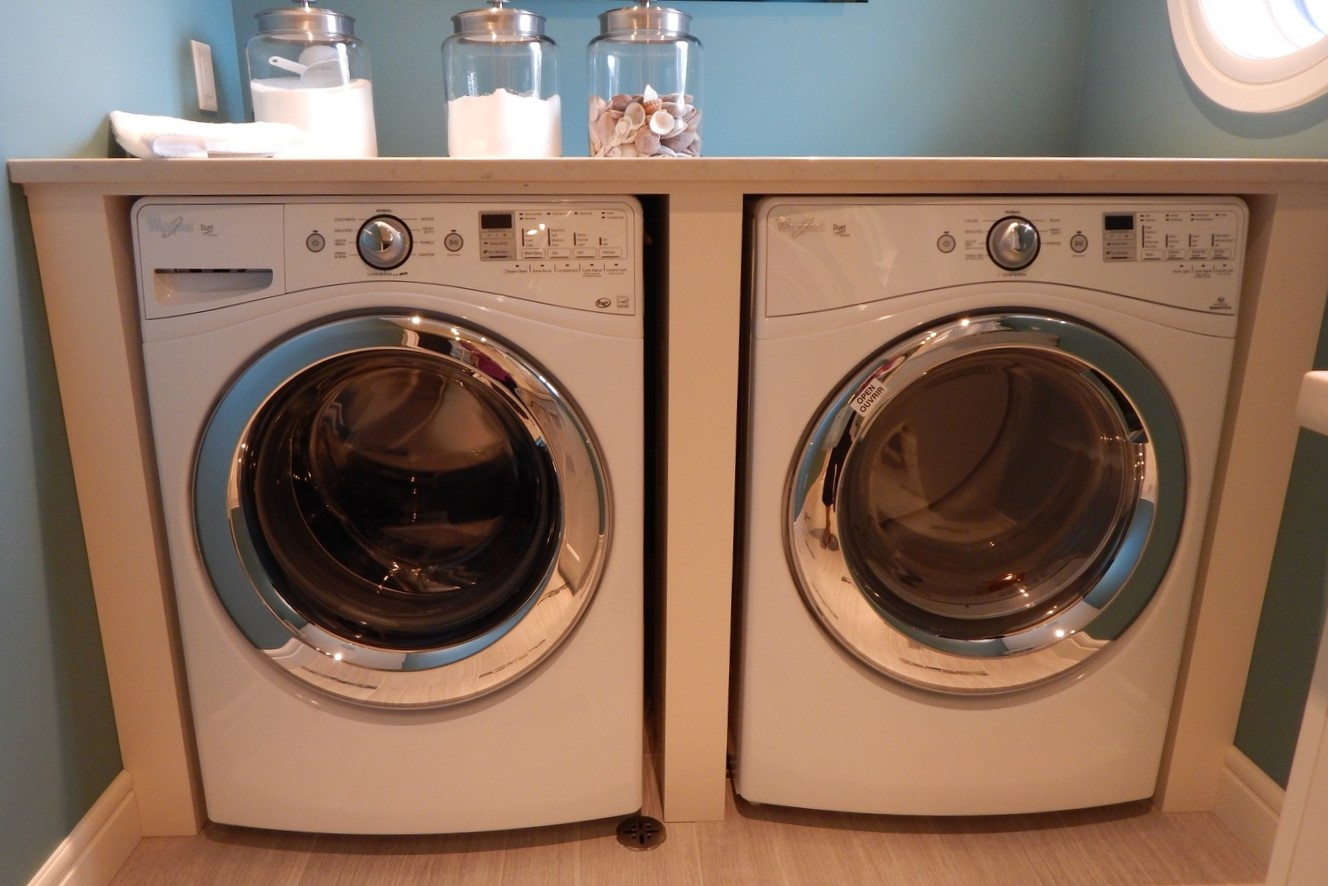
\includegraphics[width=0.5\textwidth]{fig/lec01/Home_appliance.jpg}
			\caption{Home appliances (source: \href{https://pxhere.com/de/photo/863012}{pxhere}, \href{https://creativecommons.org/publicdomain/zero/1.0/}{CC0~1.0})}
		\end{subfigure}
		\pause
		\hfill
		\begin{subfigure}[b]{0.49\textwidth}
			\centering
			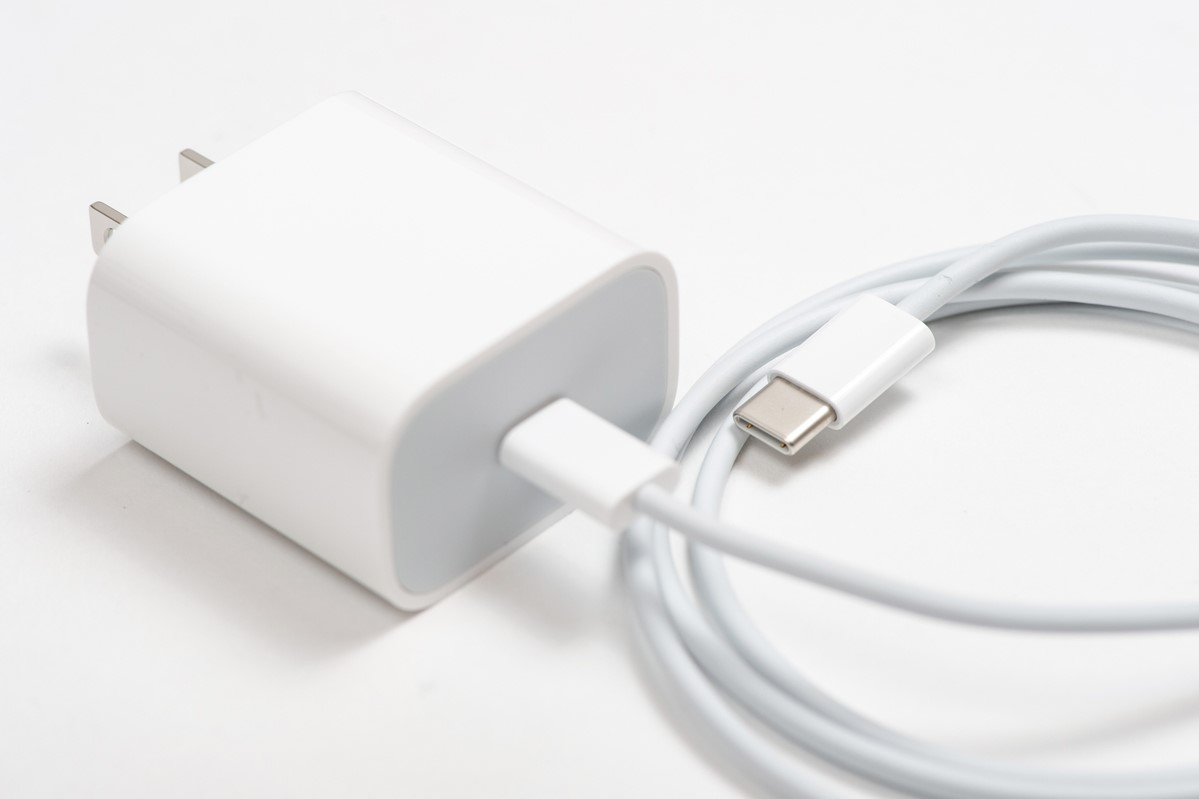
\includegraphics[width=0.5\textwidth]{fig/lec01/Smartphone_charger.jpg}
			\caption{Smartphone charger (source: \href{https://www.rawpixel.com/image/5923136/photo-image-phone-public-domain-white}{rawpixel}, \href{https://creativecommons.org/publicdomain/zero/1.0/}{CC0~1.0})}
		\end{subfigure}
		\pause
		\\
		\begin{subfigure}[b]{0.49\textwidth}
			\centering
			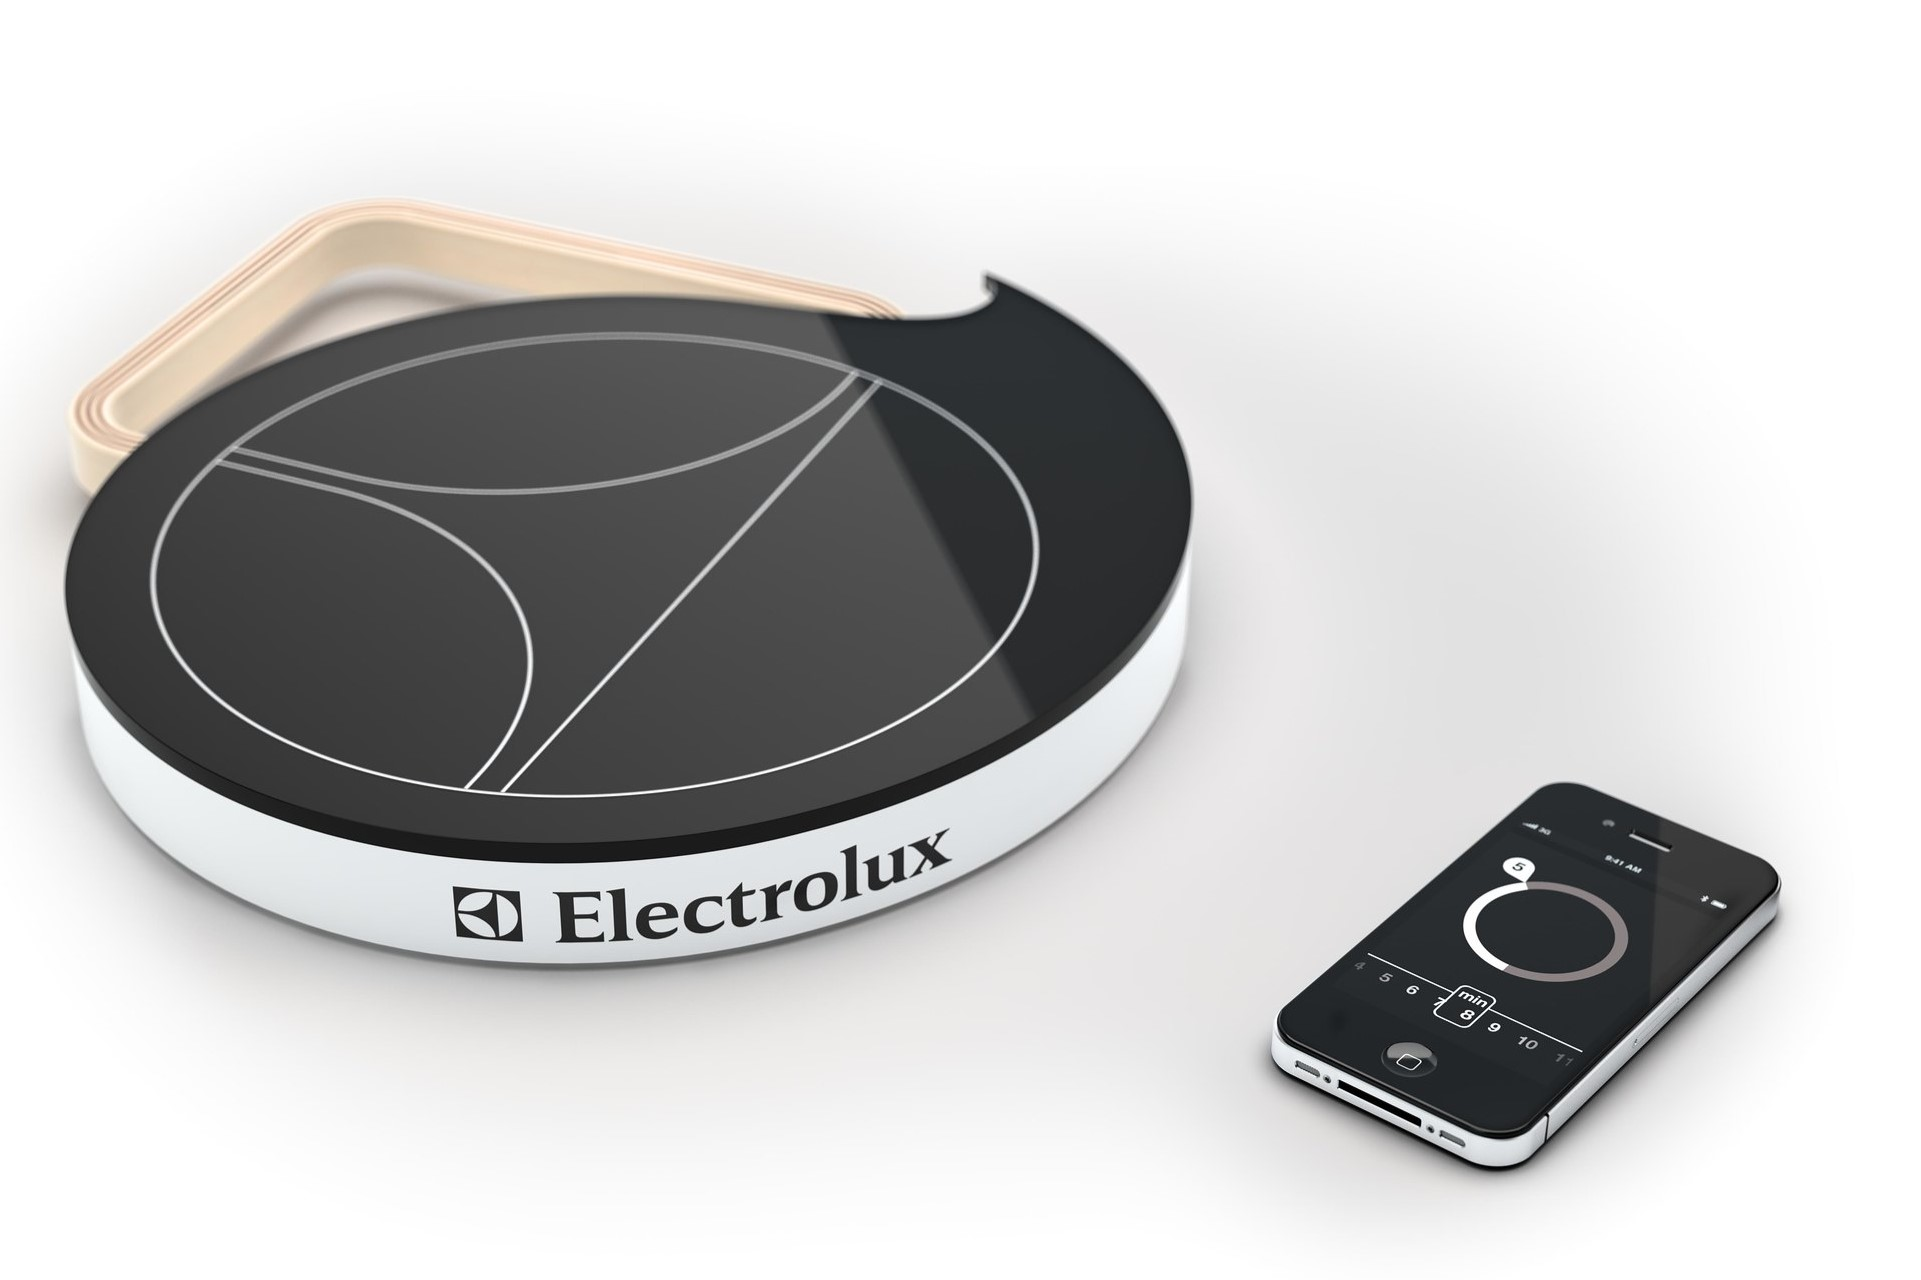
\includegraphics[width=0.5\textwidth]{fig/lec01/Induction_plate.jpg}
			\caption{Induction plate (source: \href{https://www.flickr.com/photos/electrolux-design-lab/6035618944}{flickr}, Electrolux, \href{https://creativecommons.org/licenses/by-nc/2.0/}{CC~BY-SA-NC~2.0})}
		\end{subfigure}
		\pause
		\hfill
		\begin{subfigure}[b]{0.49\textwidth}
			\centering
			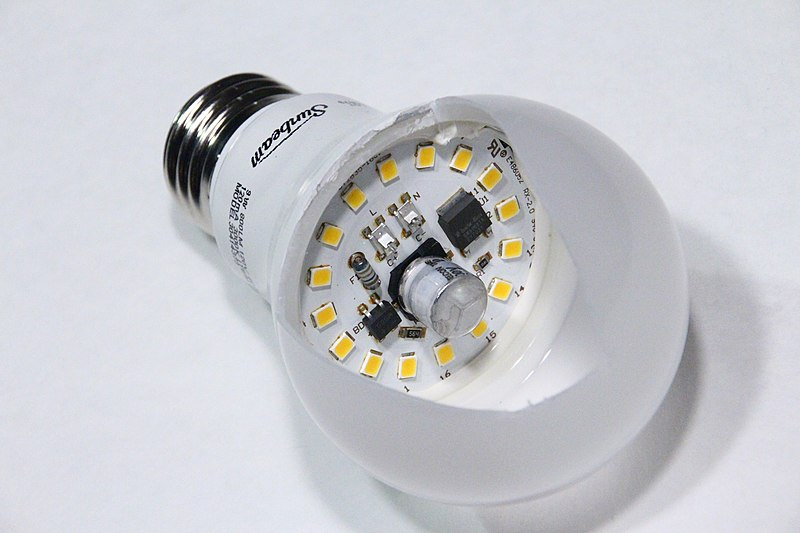
\includegraphics[width=0.5\textwidth]{fig/lec01/LED_light_bulb.jpg}
			\caption{LED rectifier (source: \href{https://commons.wikimedia.org/wiki/File:LED-E27-Light-Bulb-1134.jpg}{Wikimedia Commons}, D.~Tribble, \href{https://creativecommons.org/licenses/by-sa/4.0/deed.en}{CC~BY-SA~4.0})}
		\end{subfigure}
	\end{figure}
\end{frame}

%%%%%%%%%%%%%%%%%%%%%%%%%%%%%%%%%%%%%%%%%%%%%%%%%%%%%%%%%%%%%
%% Power electronic application examples: industrial %%
%%%%%%%%%%%%%%%%%%%%%%%%%%%%%%%%%%%%%%%%%%%%%%%%%%%%%%%%%%%%%
\begin{frame}[c]
	\frametitle{Power electronic application examples: industrial}
	\begin{figure}
		\centering
		\begin{subfigure}[b]{0.49\textwidth}
			\centering
			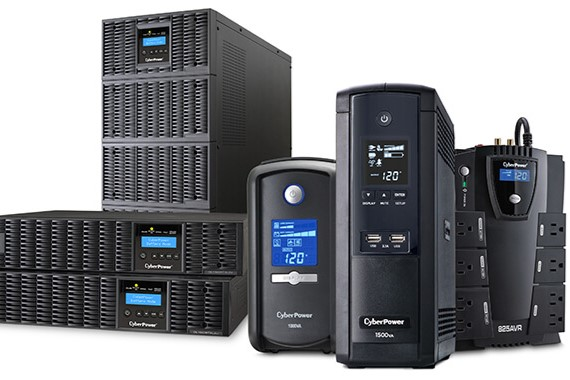
\includegraphics[width=0.5\textwidth]{fig/lec01/UPS.jpg}
			\caption{Uninterruptible power supply (source: \href{https://commons.wikimedia.org/wiki/File:CyberPower_UPS_Systems.jpg}{Wikimedia Commons}, Stevebwallace, \href{https://creativecommons.org/licenses/by-sa/4.0/deed.en}{CC~BY-SA~4.0})}
		\end{subfigure}
		\pause
		\hfill
		\begin{subfigure}[b]{0.49\textwidth}
			\centering
			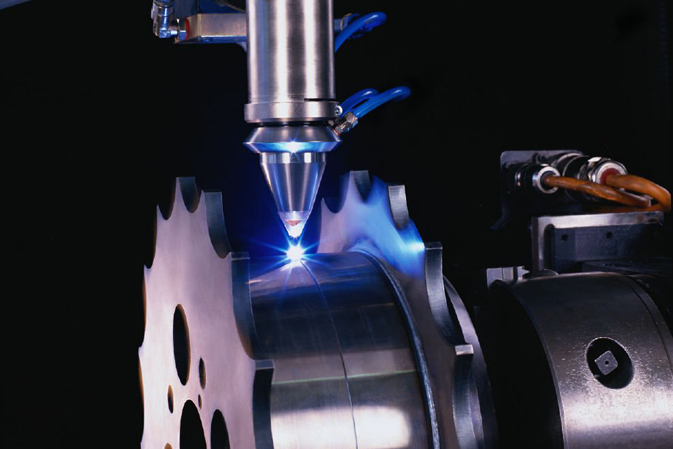
\includegraphics[width=0.5\textwidth]{fig/lec01/Welding.jpg}
			\caption{Welding power supply (source: \href{https://commons.wikimedia.org/wiki/File:Trumpf_laserschweissen.jpg}{Wikimedia Commons}, Trumpf GmbH, \href{https://creativecommons.org/licenses/by-sa/3.0/deed.en}{CC~BY-SA~3.0})}
		\end{subfigure}
		\pause
		\\
		\begin{subfigure}[b]{0.49\textwidth}
			\centering
			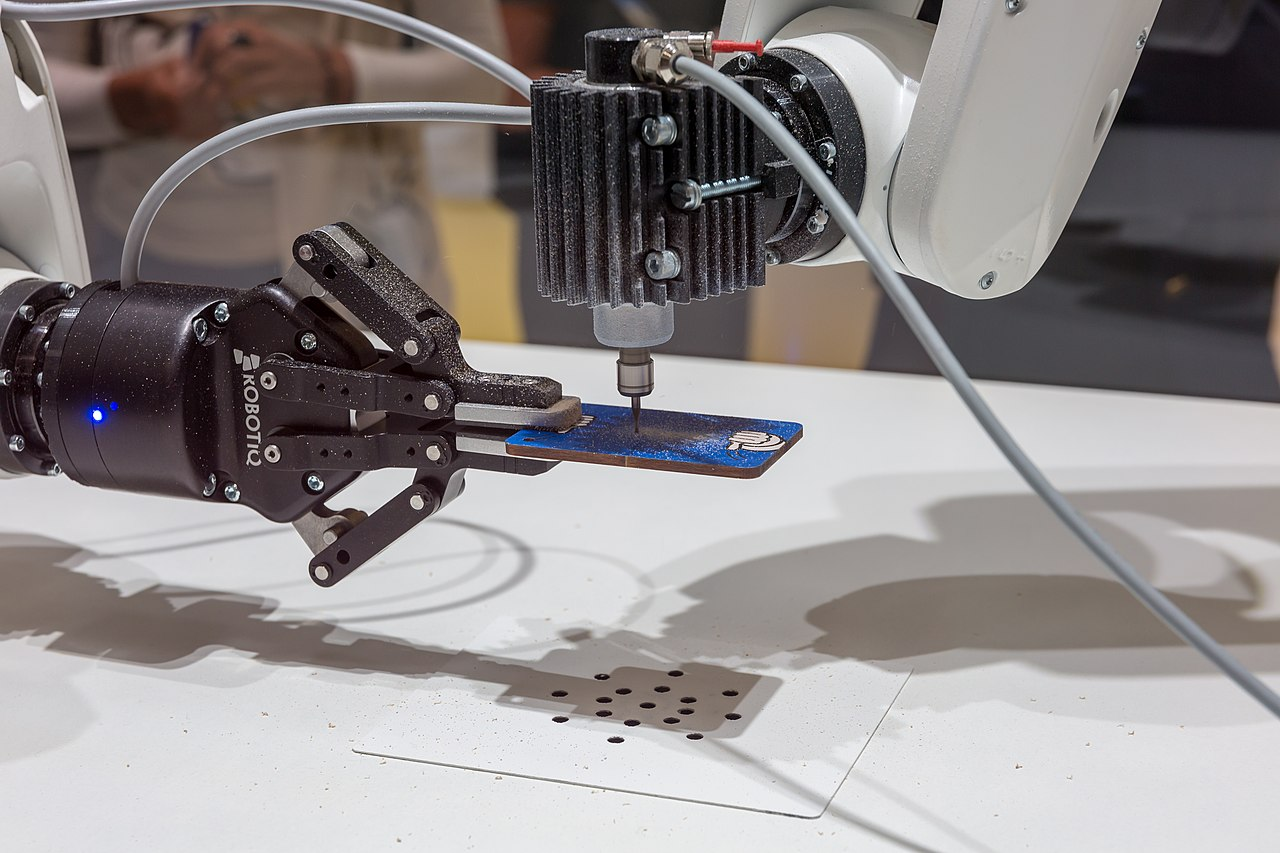
\includegraphics[width=0.5\textwidth]{fig/lec01/Robot.jpg}
			\caption{Industrial drives / automation (source: \href{https://de.m.wikipedia.org/wiki/Datei:Paris_Motor_Show_2018,_Paris_\%281Y7A1752\%29.jpg}{Wikimedia Commons}, M.~Blume, \href{https://creativecommons.org/licenses/by-sa/4.0/deed.de}{CC~BY-SA~4.0})}
		\end{subfigure}
		\pause
		\hfill
		\begin{subfigure}[b]{0.49\textwidth}
			\centering
			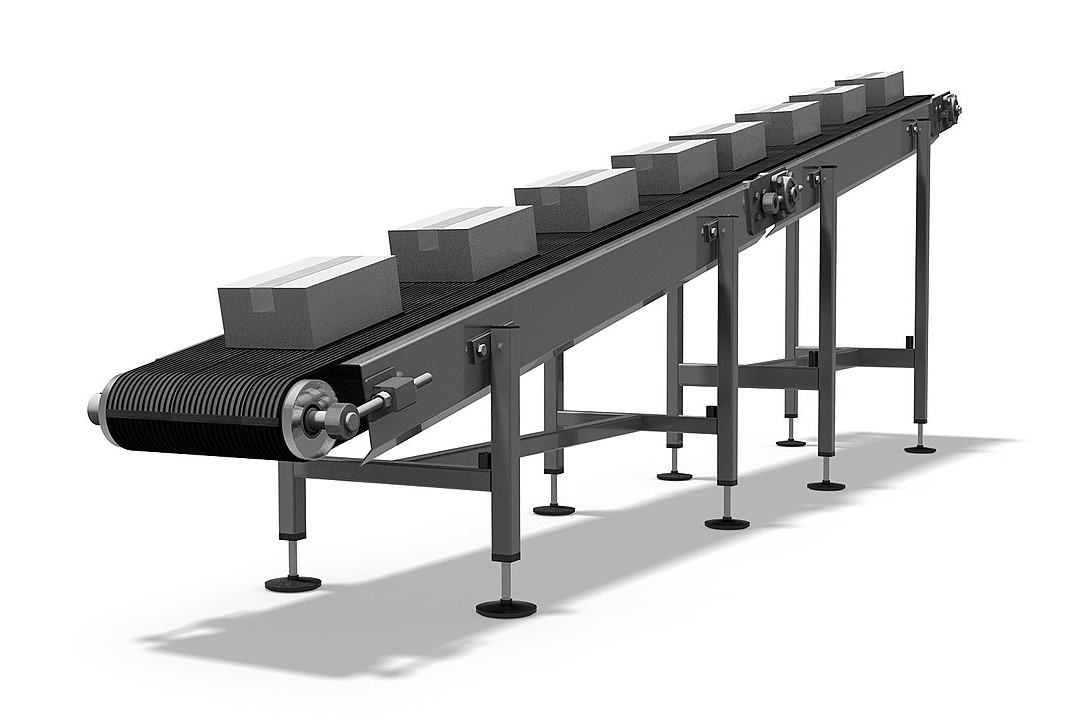
\includegraphics[width=0.5\textwidth]{fig/lec01/Conveyor.jpg}
			\caption{Conveyor belt drive (source: \href{https://commons.wikimedia.org/wiki/File:Inclined-belt_conveyor.jpgg}{Wikimedia Commons},  	K.~Hannessen, \href{https://creativecommons.org/licenses/by-sa/4.0/deed.en}{CC~BY-SA~4.0})}
		\end{subfigure}
	\end{figure}
\end{frame}

%%%%%%%%%%%%%%%%%%%%%%%%%%%%%%%%%%%%%%%%%%%%%%%%%%%%%%%%%%%%%
%% Power electronic application examples: energy system %%
%%%%%%%%%%%%%%%%%%%%%%%%%%%%%%%%%%%%%%%%%%%%%%%%%%%%%%%%%%%%%
\begin{frame}[c]
	\frametitle{Power electronic application examples: energy system}
	\begin{figure}
		\centering
		\begin{subfigure}[b]{0.49\textwidth}
			\centering
			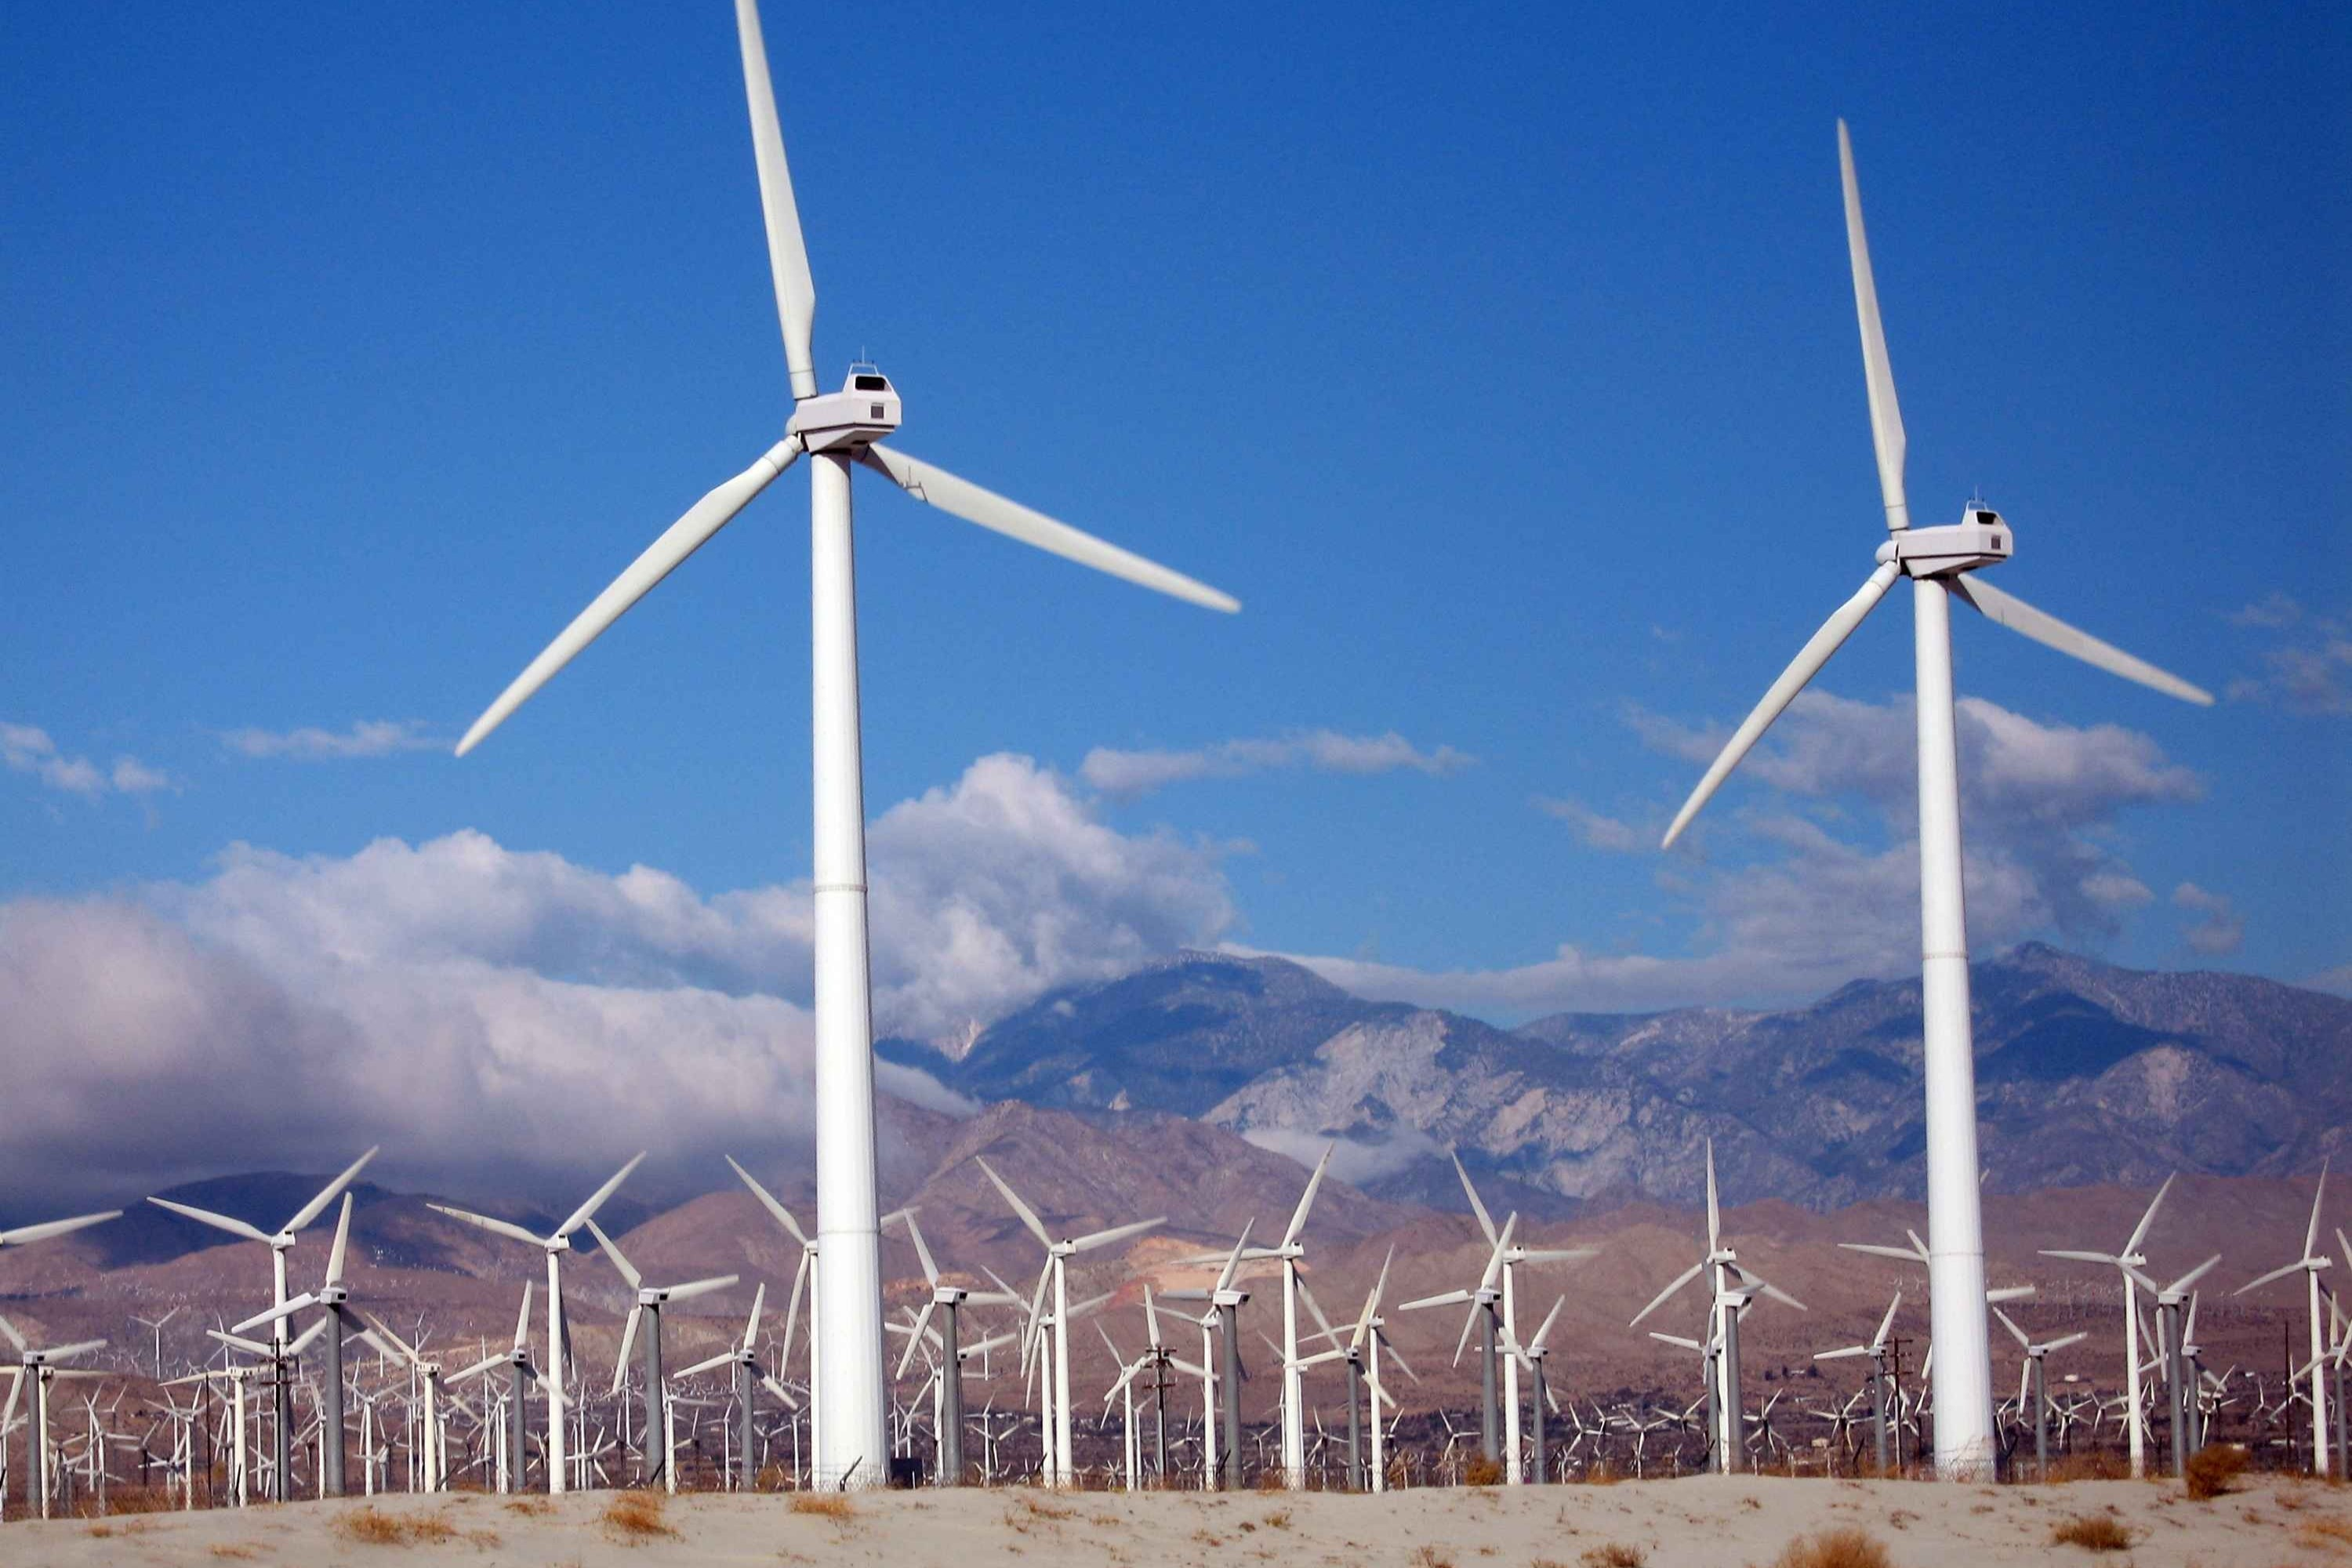
\includegraphics[width=0.5\textwidth]{fig/lec01/sky-farm-windmill.jpg}
			\caption{Wind power plants (source: \href{https://pxhere.com/en/photo/954757}{pxhere}, \href{https://creativecommons.org/publicdomain/zero/1.0/}{CC0~1.0})}
		\end{subfigure}
		\pause
		\hfill
		\begin{subfigure}[b]{0.49\textwidth}
			\centering
			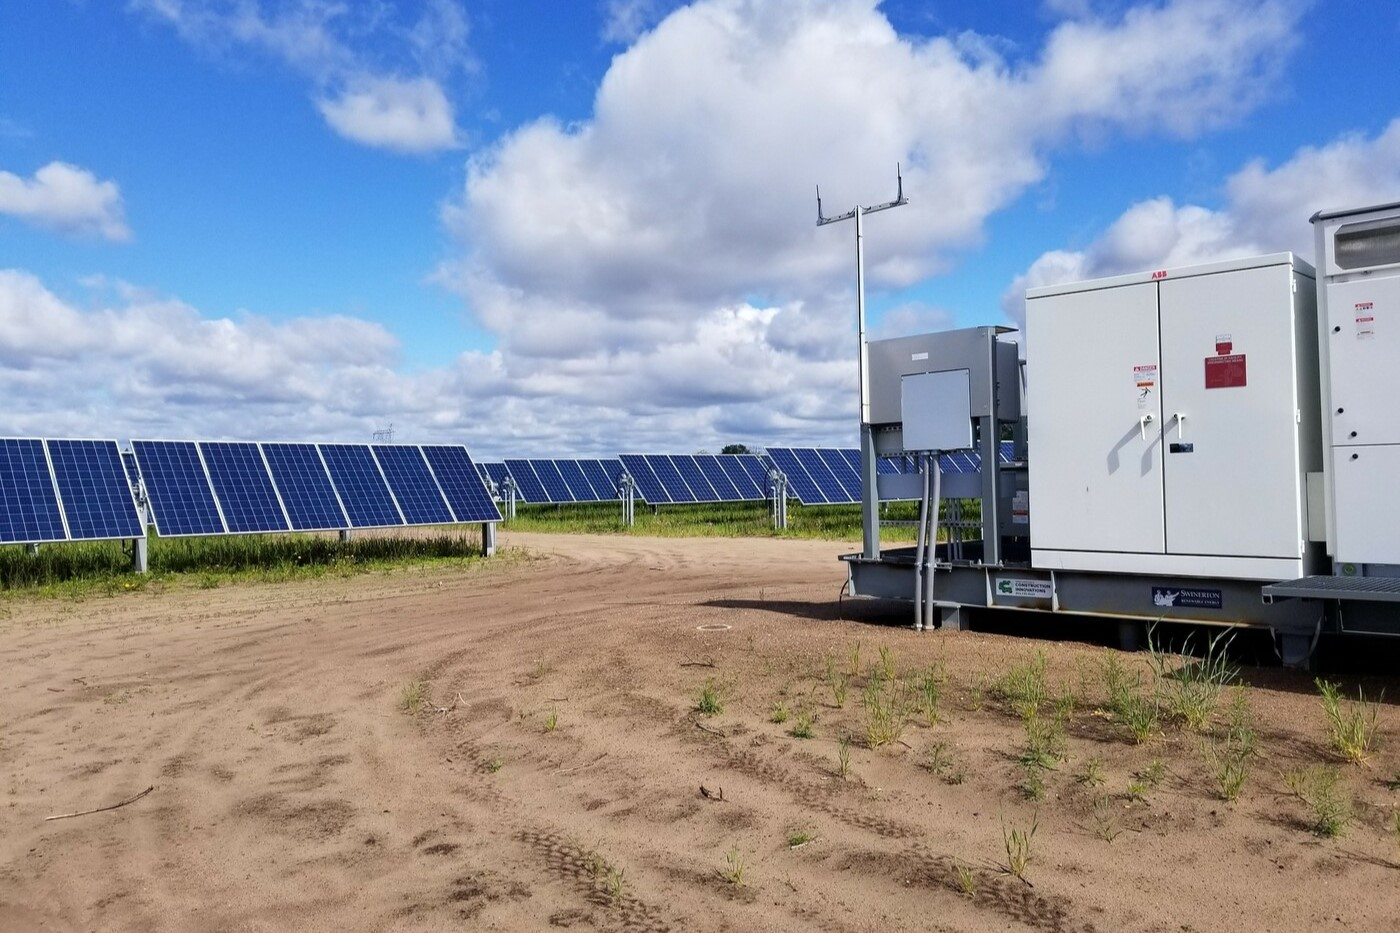
\includegraphics[width=0.5\textwidth]{fig/lec01/PV_field.jpg}
			\caption{PV power plants (source: \href{https://pxhere.com/en/photo/1685464}{pxhere}, \href{https://creativecommons.org/publicdomain/zero/1.0/}{CC0~1.0})}
		\end{subfigure}
		\pause
		\\
		\begin{subfigure}[b]{0.49\textwidth}
			\centering
			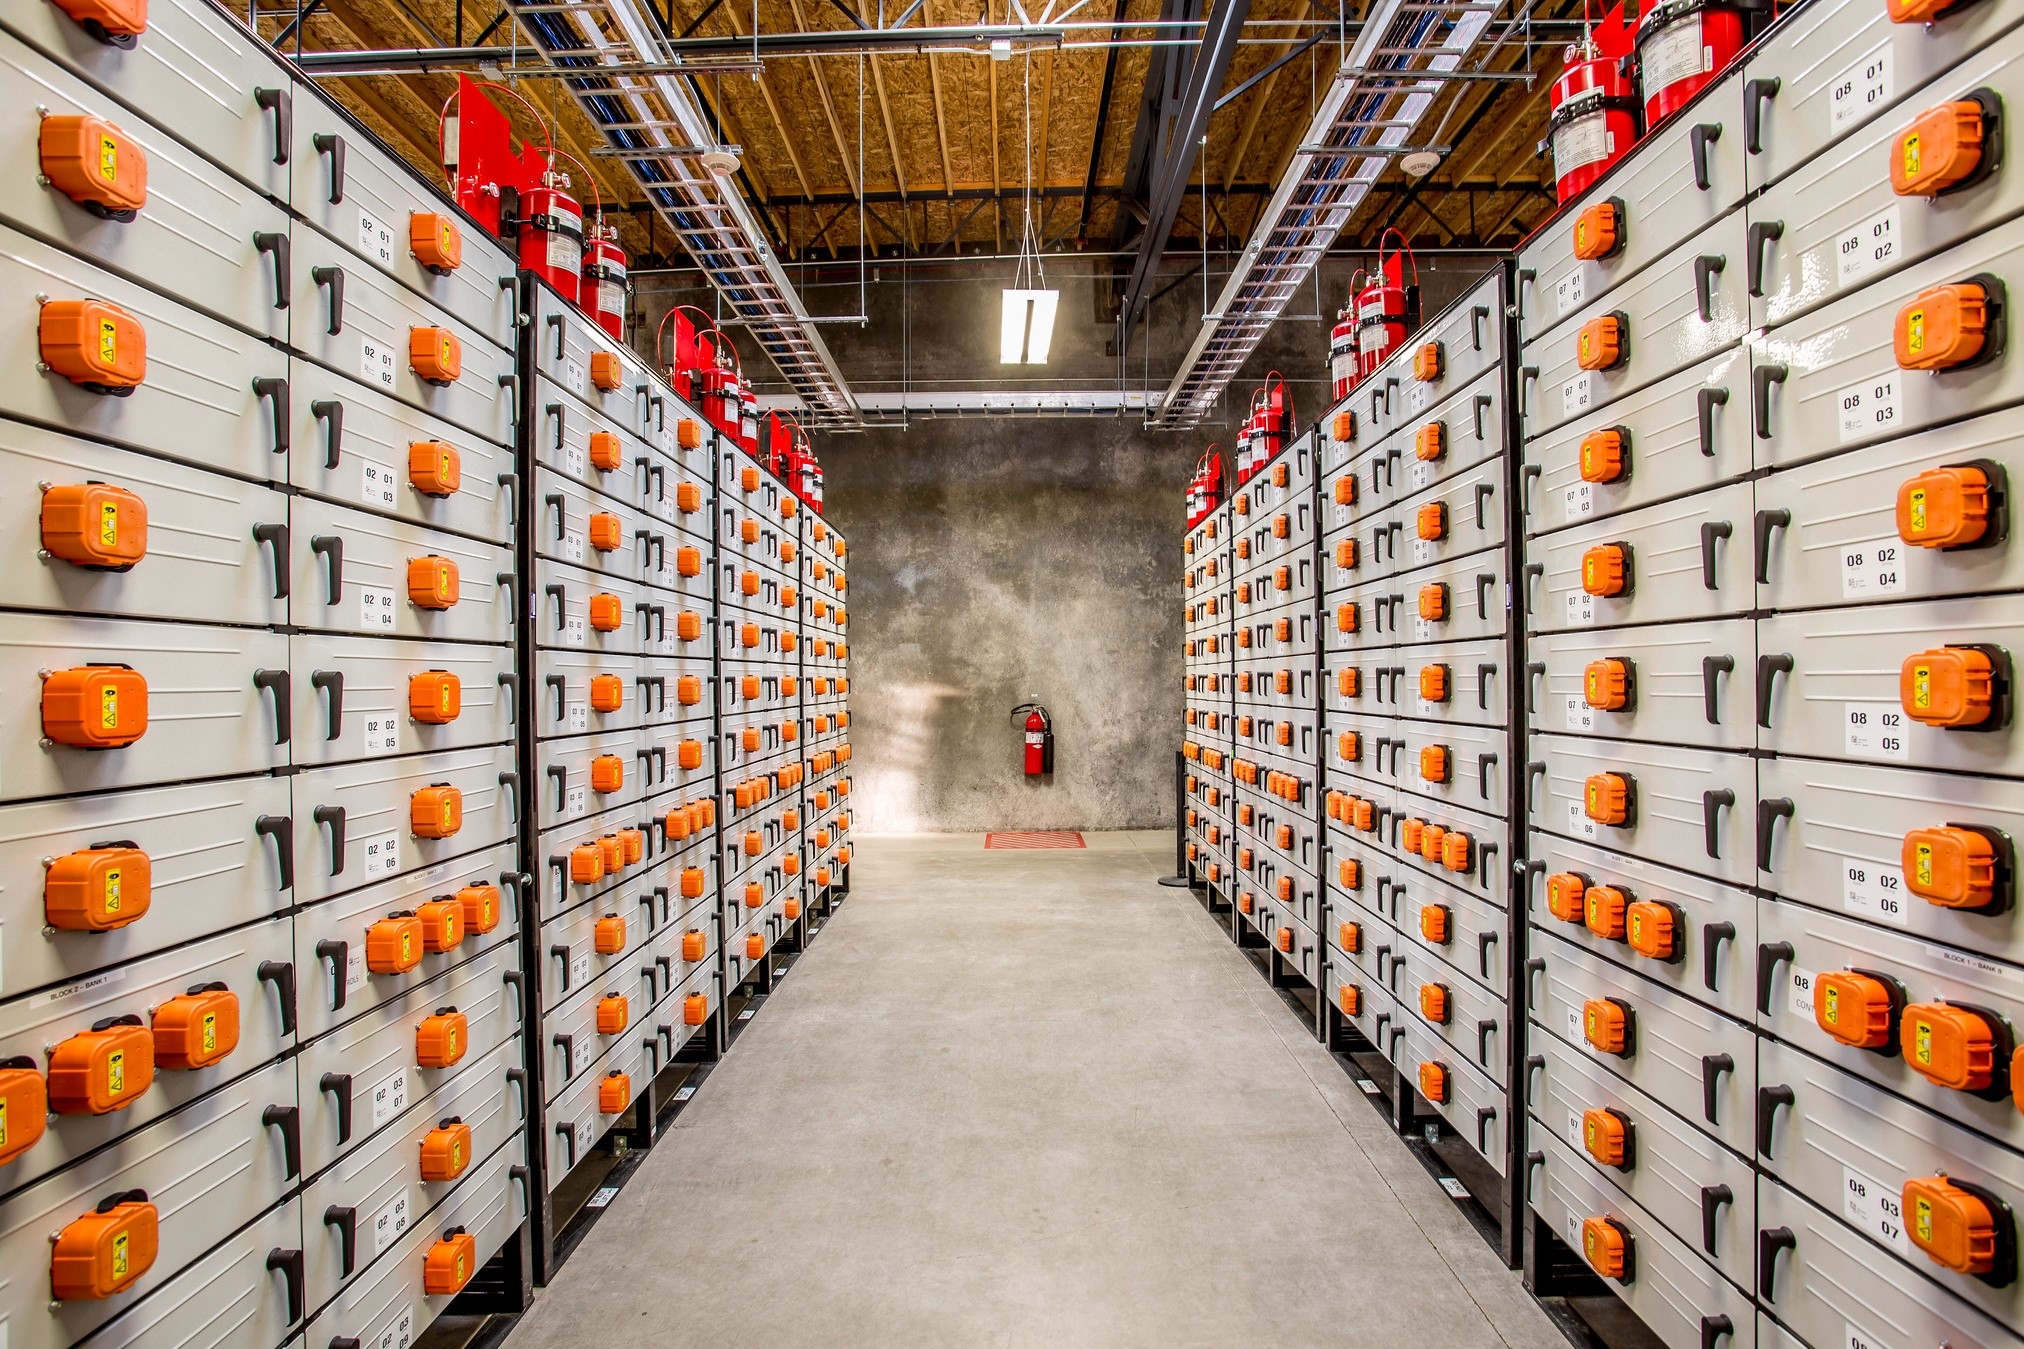
\includegraphics[width=0.5\textwidth]{fig/lec01/Battery_storage.jpg}
			\caption{Battery storage systems (source: \href{https://www.flickr.com/photos/portlandgeneralelectric/8905201835}{flickr}, 
			Portland General Electric, \href{https://creativecommons.org/licenses/by-nd/2.0/}{CC~BY-ND~2.0})}
		\end{subfigure}
		\pause
		\hfill
		\begin{subfigure}[b]{0.49\textwidth}
			\centering
			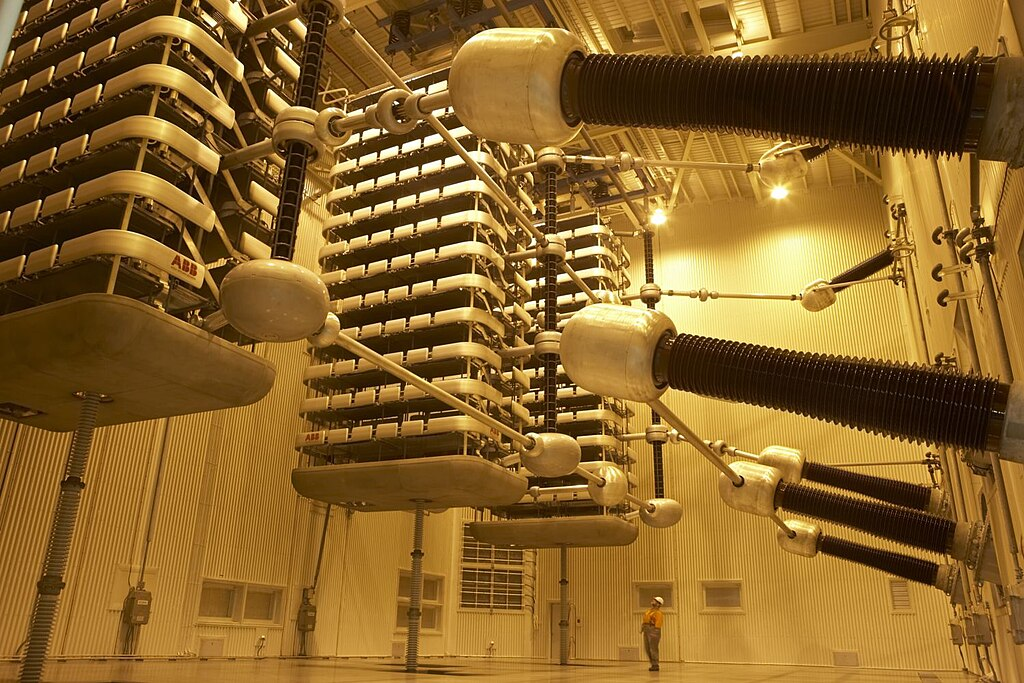
\includegraphics[width=0.5\textwidth]{fig/lec01/HVDC.jpg}
			\caption{High voltage DC transmission (source: \href{https://commons.wikimedia.org/wiki/File:Pole_2_Thyristor_Valve.jpg}{Wikimedia Commons},  	 	Marshelec, \href{https://creativecommons.org/licenses/by-sa/3.0/deed.en}{CC~BY-SA~3.0})}
		\end{subfigure}
	\end{figure}
\end{frame}

%%%%%%%%%%%%%%%%%%%%%%%%%%%%%%%%%%%%%%%%%%%%%%%%%%%%%%%%%%%%%
%% Power electronic application examples: transportation %%
%%%%%%%%%%%%%%%%%%%%%%%%%%%%%%%%%%%%%%%%%%%%%%%%%%%%%%%%%%%%%
\begin{frame}[c]
	\frametitle{Power electronic application examples: transportation}
	\begin{figure}
		\centering
		\begin{subfigure}[b]{0.49\textwidth}
			\centering
			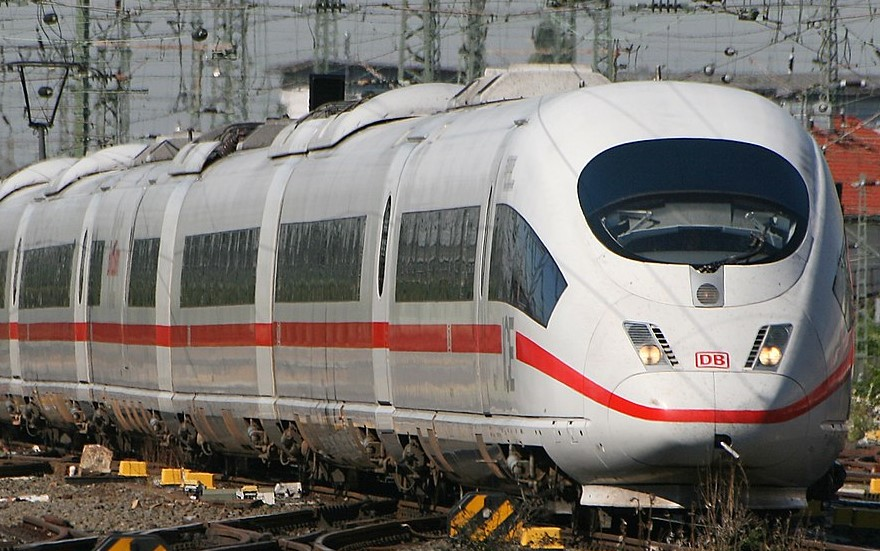
\includegraphics[width=0.5\textwidth]{fig/lec01/ICE.jpg}
			\caption{Train drive (source: \href{hhttps://commons.wikimedia.org/wiki/File:DB_AG_406_001-8.jpg}{Wikimedia Commons}, T.~Wolf, \href{https://creativecommons.org/publicdomain/zero/1.0/}{CC0~1.0})}
		\end{subfigure}
		\pause
		\hfill
		\begin{subfigure}[b]{0.49\textwidth}
			\centering
			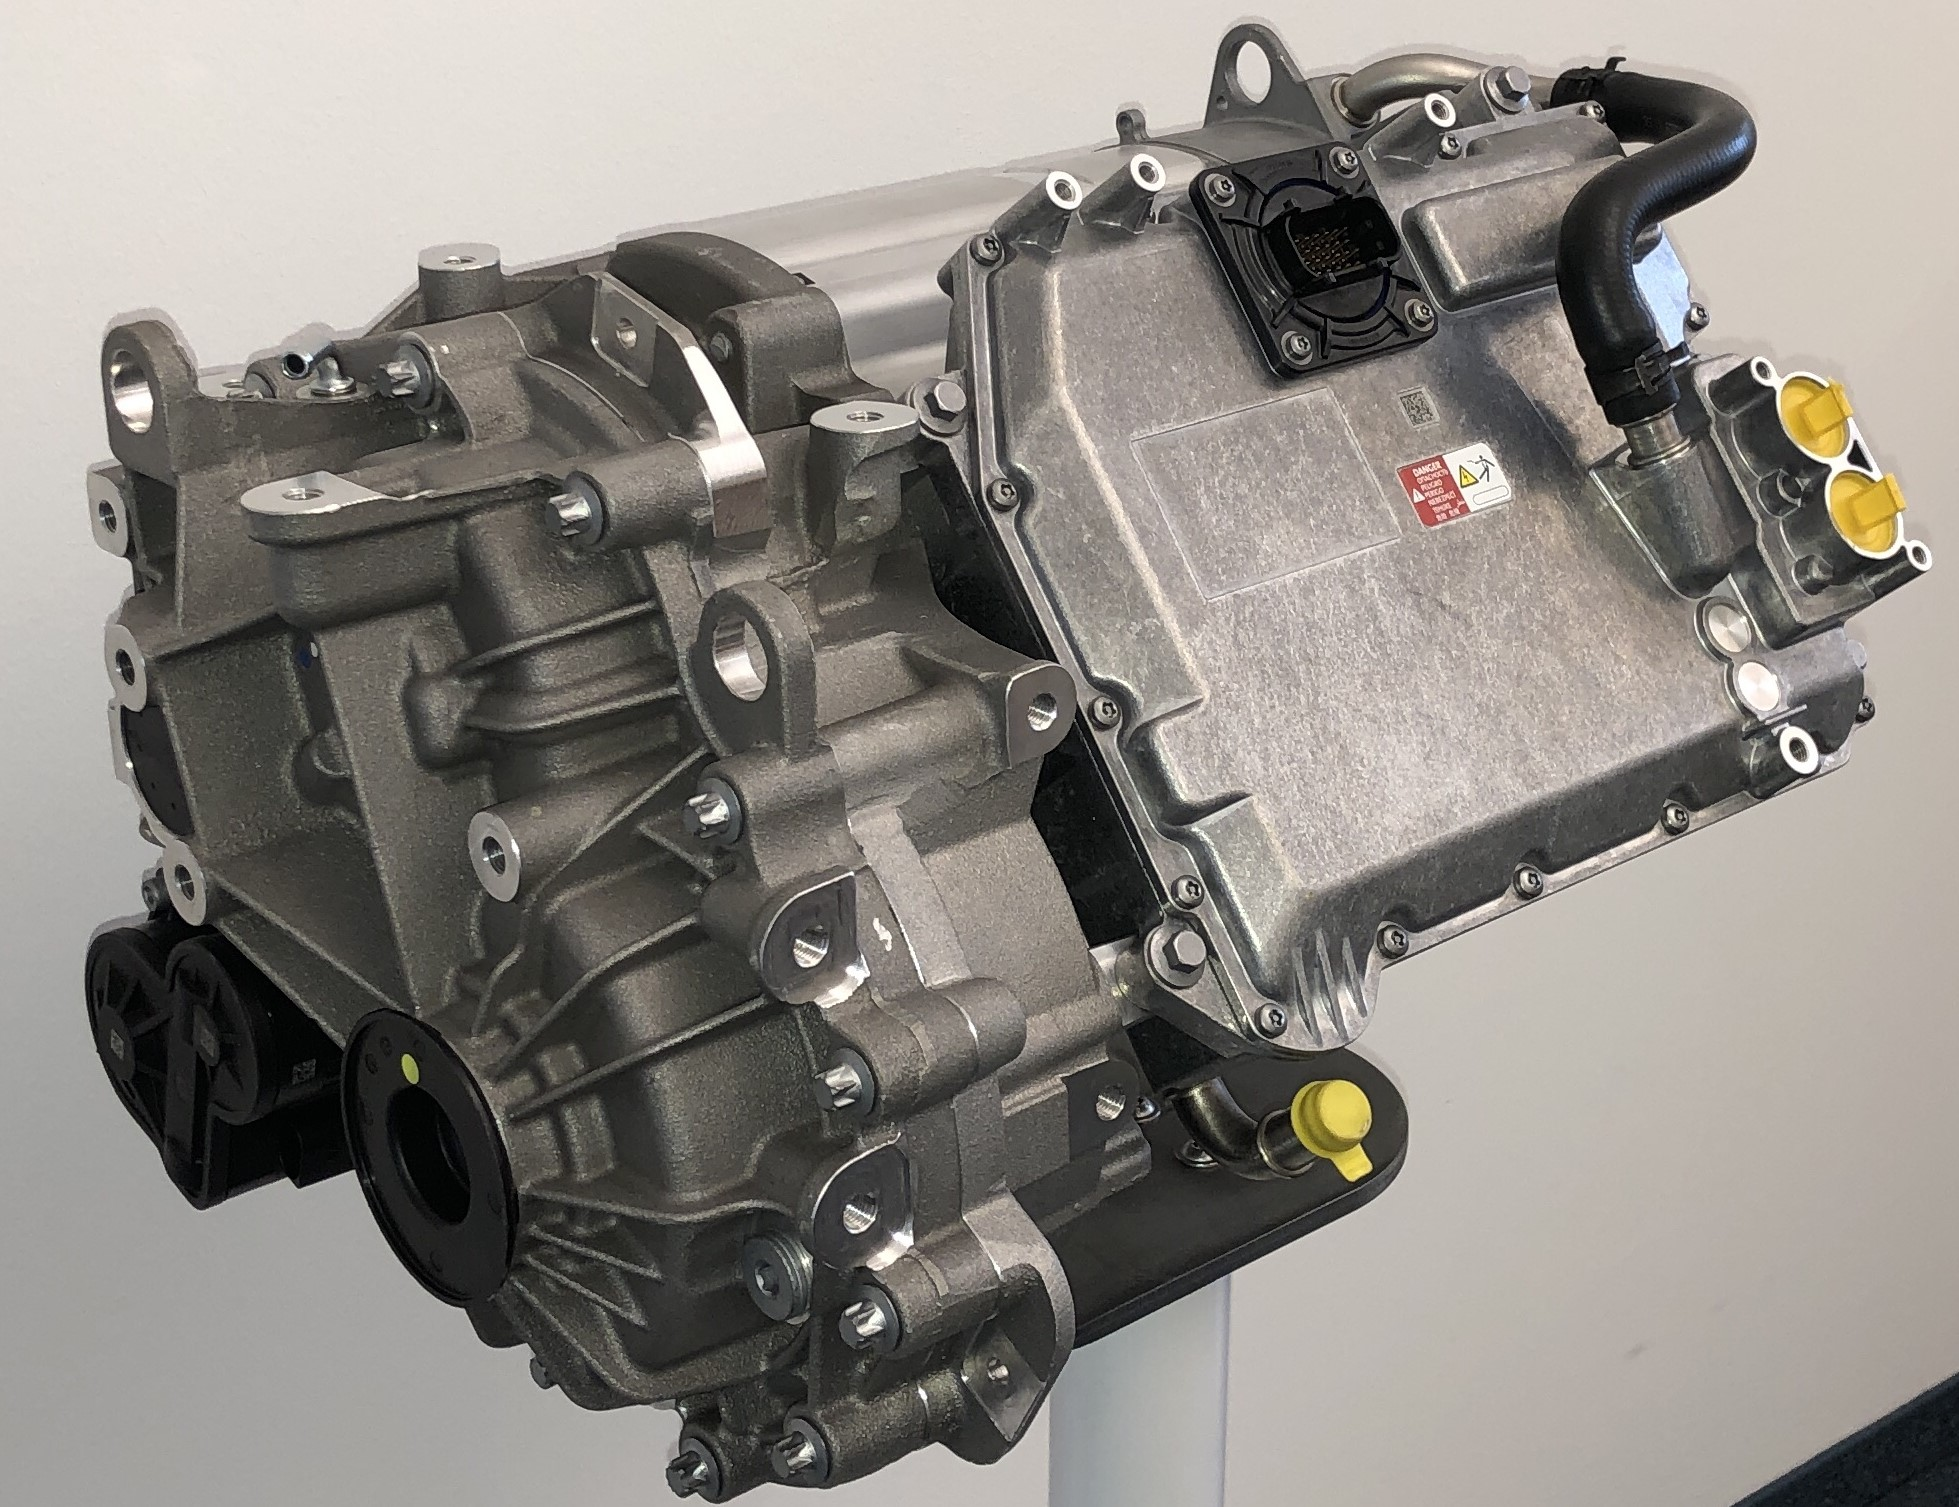
\includegraphics[width=0.5\textwidth]{fig/lec01/Drive.jpg}
			\caption{Electric vehicle drive (source: \href{https://commons.wikimedia.org/wiki/File:Vitesco_Technologies_EMR3.jpg}{Wikimedia Commons}, Caprolactam123, \href{https://creativecommons.org/licenses/by-sa/4.0/deed.en}{CC~BY-SA~4.0})}
		\end{subfigure}
		\pause
		\\
		\begin{subfigure}[b]{0.49\textwidth}
			\centering
			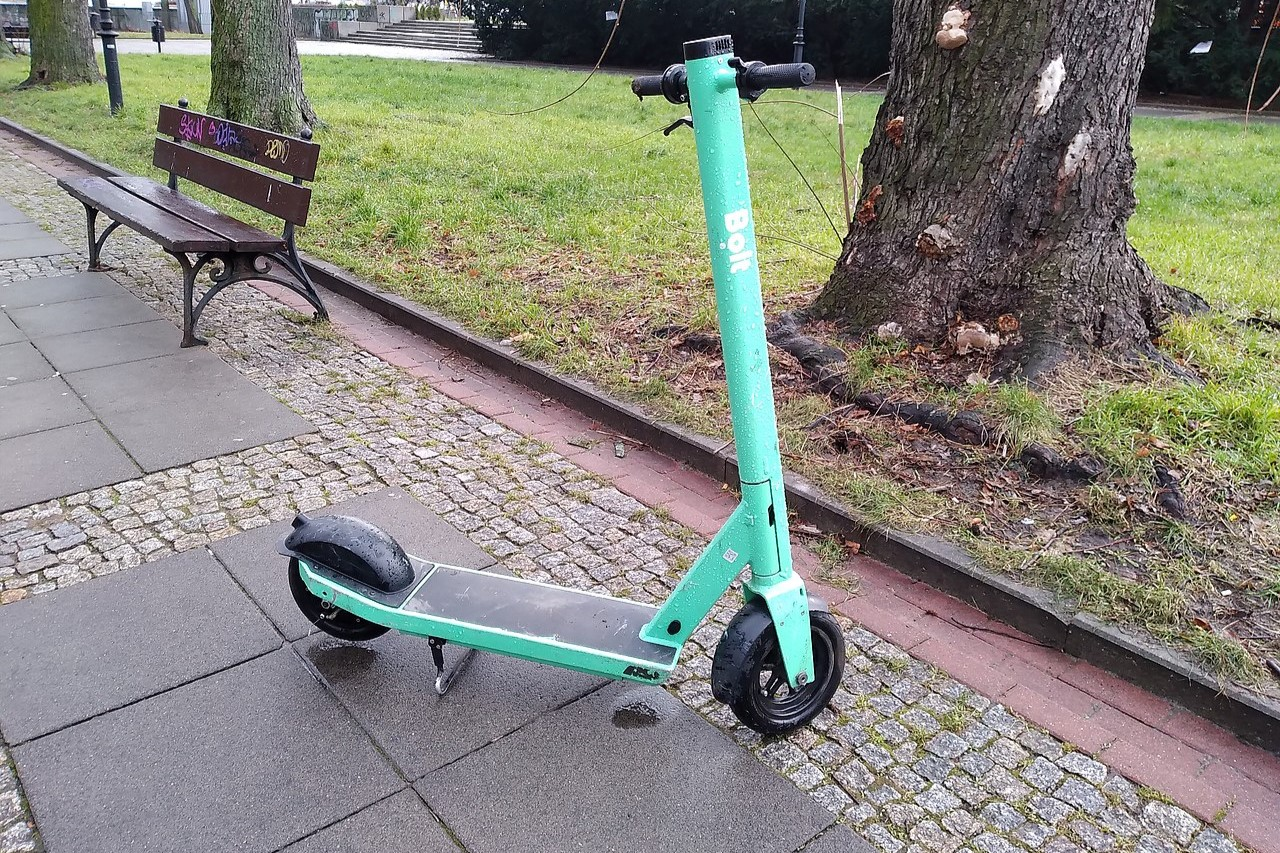
\includegraphics[width=0.5\textwidth]{fig/lec01/Scooter.jpg}
			\caption{Electric scooter (source: \href{https://commons.wikimedia.org/wiki/File:Bolt_Electric_Scooter_\%28Warsaw\%29_in_2020.03.jpg}{Wikimedia Commons}, Raju, \href{https://creativecommons.org/licenses/by-sa/4.0/deed.en}{CC~BY-SA~4.0})}
		\end{subfigure}
		\pause
		\hfill
		\begin{subfigure}[b]{0.49\textwidth}
			\centering
			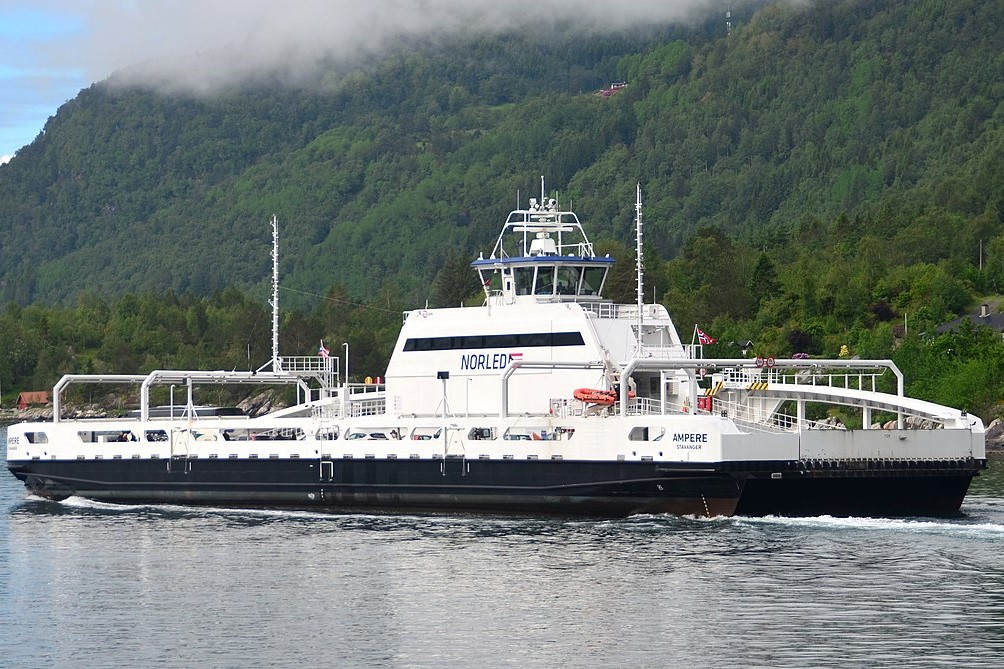
\includegraphics[width=0.5\textwidth]{fig/lec01/Electric_ship.jpg}
			\caption{Electic ship (source: \href{https://commons.wikimedia.org/wiki/File:Ferry_Ampere_Sognefjord.jpg}{Wikimedia Commons},  	 	Wikimalte, \href{https://creativecommons.org/licenses/by-sa/4.0/deed.en}{CC~BY-SA~4.0})}
		\end{subfigure}
	\end{figure}
\end{frame}

%%%%%%%%%%%%%%%%%%%%%%%%%%%%%%%%%%%%%%%%%%%%%%%%%%%%%%%%%%%%%
%% A broad range of nominal power ratings %%
%%%%%%%%%%%%%%%%%%%%%%%%%%%%%%%%%%%%%%%%%%%%%%%%%%%%%%%%%%%%%
\begin{frame}[c]
	\frametitle{A broad range of nominal power ratings}
	\vspace{0.3cm}
	\begin{figure}
		\centering
		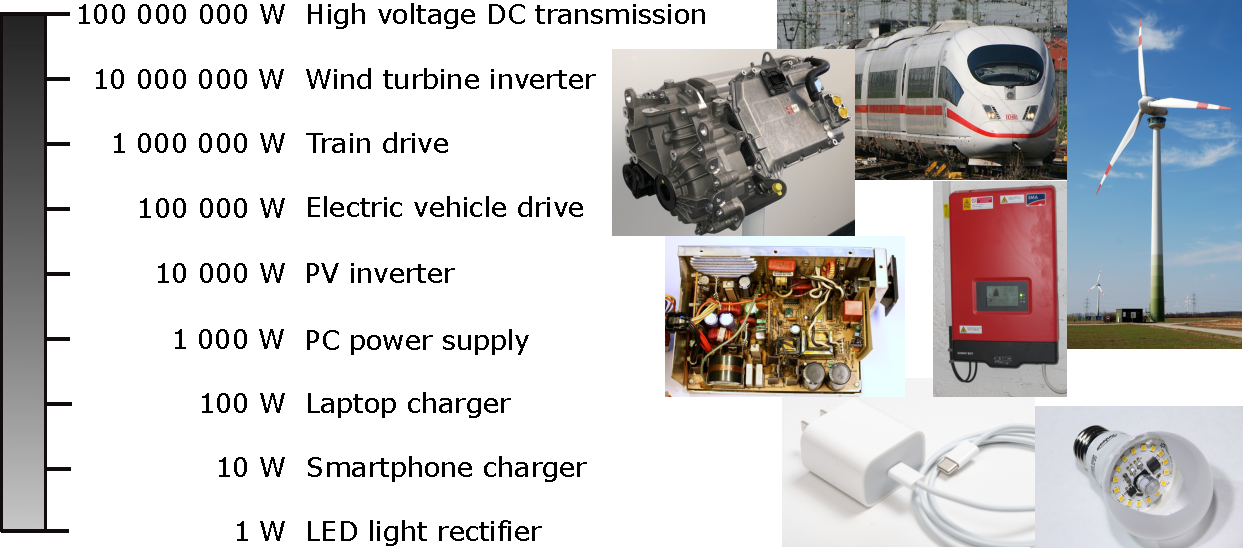
\includegraphics[height=0.7\textheight]{fig/lec01/Power_Classes_Examples.pdf}
		\caption{Power range overview (figure sources: \href{https://commons.wikimedia.org/wiki/File:DB_AG_406_001-8.jpg}{T. Wolf}, \href{https://commons.wikimedia.org/wiki/File:Wind_turbine_with_observation_deck_bruck_an_der_leitha.jpg}{KoeppiK}, \href{https://commons.wikimedia.org/wiki/File:Vitesco_Technologies_EMR3.jpg}{Caprolactam123}, \href{https://commons.wikimedia.org/wiki/File:Installation_of_solar_PV_panels_-_inverter_-_geograph.org.uk_-_2624304.jpg}{D. Hawgood}, \href{https://commons.wikimedia.org/wiki/File:IBM_PC_XT_5160_Power_Supply.jpg}{Mister rf}, \href{https://commons.wikimedia.org/wiki/File:LED-E27-Light-Bulb-1134.jpg}{D.~Tribble} and \href{https://www.rawpixel.com/image/5923136/photo-image-phone-public-domain-white}{rawpixel} under varying CC licenses) }
		\label{Power_Classes_Examples}
	\end{figure}
\end{frame}

%%%%%%%%%%%%%%%%%%%%%%%%%%%%%%%%%%%%%%%%%%%%%%%%%%%%%%%%%%%%%
%% Typical power electronic objectives %%
%%%%%%%%%%%%%%%%%%%%%%%%%%%%%%%%%%%%%%%%%%%%%%%%%%%%%%%%%%%%%
\begin{frame}[c]
	\frametitle{Typical power electronic objectives}
	\begin{figure}
		\begin{tikzpicture}
			\begin{axis}[
				height=.70\textheight,
				ylabel={Efficiency},
				xlabel={Power density},
				zlabel={Costs / ressources},
				xlabel style={sloped},
				ylabel style={sloped}, 
				xticklabel style = {yshift=0.2cm, rotate=25},
				view={70}{25},
				grid,
				ymax = 1,
				xmax = 1,
				zmax = 1,
				xtick distance = 0.25,
				ytick distance = 0.25,
				ztick distance = 0.25
			]
			\addplot3[
				mesh,
				samples=20,
				domain=0:1,
				draw = signalalpha
			](
				{sqrt(1-x^2) * cos(deg(y))},
				{sqrt( 1-x^2 ) * sin(deg(y))},
				{x}
			);
			\end{axis}
		\end{tikzpicture}
		\caption{Illustration of typical, conflicting power electronic (normalized) objectives via a Pareto front}
		\label{fig:power_electronic_objectives}
	\end{figure}
\end{frame}

%%%%%%%%%%%%%%%%%%%%%%%%%%%%%%%%%%%%%%%%%%%%%%%%%%%%%%%%%%%%%
%% Subsection: Energy, work, and power %%
%%%%%%%%%%%%%%%%%%%%%%%%%%%%%%%%%%%%%%%%%%%%%%%%%%%%%%%%%%%%%
\subsection{Energy, work, and power}

%%%%%%%%%%%%%%%%%%%%%%%%%%%%%%%%%%%%%%%%%%%%%%%%%%%%%%%%%%%%%
%% Terminology: work vs. energy%%
%%%%%%%%%%%%%%%%%%%%%%%%%%%%%%%%%%%%%%%%%%%%%%%%%%%%%%%%%%%%%
\begin{frame}[c]
	\frametitle{Terminology: work vs. energy}
	\begin{columns}
		\begin{column}{0.5\textwidth}
			\onslide<2->{
				\begin{varblock}{Work}
					Work is the integral of the power over a time integral (or force over distance) and is a measure of the energy transfer.
				\end{varblock}
			}
		\end{column}
		\begin{column}{0.5\textwidth}
			\onslide<1->{
				\begin{varblock}{Energy}
					Energy is the capacity to do work, that is, a quantity depending on the state of a system at a given point of time.				
				\end{varblock}
			}
		\end{column}
	\end{columns}
	\vspace{0.5cm}
	\begin{figure}
		\begin{tikzpicture}
			\onslide<1->{\node[draw, bubble, minimum width = 8em, minimum height = 5em] (energy) at (0,0) {\large Energy};}
			\onslide<3->{
				\coordinate (loss) at (4.5,-1.25);
				\node[draw, bubble] (energy2) at (6,0) {\large Energy};
				}
			\begin{scope}[on background layer]
				\onslide<2->\draw[-{Latex[length=4mm, width=8mm]}, line width=4mm] (energy.mid) -- node[above, midway, name = work] {Work} (energy2);
				\onslide<3->{
					\draw[-{Latex[length=4mm, width=8mm]}, line width=2mm, color=signaldelta, transform canvas={yshift=-3mm}] (energy.mid) --  (3,0) to [out=0,in=120] (loss.south) ;
					\node[below, transform canvas={yshift=-3mm}] at (loss) {\color{signaldelta} \large Heat};
					\node[below=of work, yshift = 6mm, color=signaldelta] {Losses};
				}
			\end{scope}
		\end{tikzpicture}
		\vspace{0.75cm}
		\onslide<3->{\caption{Illustration addressing the work vs. energy terminology (simplified Sankey diagram)}}
		\label{fig:work_vs_energy}
	\end{figure}
\end{frame}

%%%%%%%%%%%%%%%%%%%%%%%%%%%%%%%%%%%%%%%%%%%%%%%%%%%%%%%%%%%%%
%% Power Power balance of an electrical energy conversion system %%
%%%%%%%%%%%%%%%%%%%%%%%%%%%%%%%%%%%%%%%%%%%%%%%%%%%%%%%%%%%%%
\begin{frame}
	\frametitle{Power balance of an electrical energy conversion system}
	\begin{figure}
		\begin{tikzpicture}[auto, node distance = 1.5cm and 2cm]
			\draw
				node [input, name = input] {}
				node [bubble, right = of input, minimum height = 4em] (pc) {\large Power converter}
				node [output, name = output, right = of pc] {}
				node [output, name = losses, below = of pc] {};
				\draw[-{Latex[length=4mm, width=8mm]}, line width=3mm] (input) -- node[below, midway, align=left, name = input2] {Electrical\\input power} (pc);
			\onslide<3->{\node[overlay, bubble, right = of input, minimum height = 4em, pin=80:Change of stored energy $ \frac{\mathrm{d}}{\mathrm{d}t}E_\mathrm{i}(t)$] {\large Power converter};}
			\begin{scope}[on background layer]
				\onslide<4->{\draw[-{Latex[length=4mm, width=8mm]}, line width=3mm] (pc.mid) -- node[below, near end, align=left, name=output2] {Electrical\\output power} (output);}
				\onslide<2->{\draw[-{Latex[length=4mm, width=8mm]}, line width=3mm, color=signaldelta] (pc.mid) -- node[right, yshift=-2.5mm, name = losses2] {Losses} (losses);}
			\end{scope}
			\onslide<2->{\node[left=of losses2, color=signaldelta, xshift = 1.8cm] {$P_\mathrm{l}(t)$};}
			\onslide<4->{\node[above=of output2.mid,, align=center, xshift = -0.3cm, yshift = -5mm] {$P_\mathrm{out}(t)$};}
			\node[above=of input2.mid,, align=center, xshift = -0.3cm, yshift = -5mm] {$P_\mathrm{in}(t)$};
		\end{tikzpicture}
		\onslide<4->{\caption{Power balance of an energy conversion system}}
		\label{fig:power_balance_energy_conversion}
	\end{figure}
	\vspace{-0.5cm}
	The \hl{power balance}
	\begin{equation}
		\onslide<1->{P_\mathrm{in}(t)} \onslide<2->{= P_\mathrm{l}(t)}  \onslide<3->{+ \frac{\mathrm{d}}{\mathrm{d}t}E_\mathrm{i}(t)} \onslide<4->{+ P_\mathrm{out}(t)}
	\end{equation}
	must hold for any point in time as energy is conserved, that is, not created or destroyed.
\end{frame}

%%%%%%%%%%%%%%%%%%%%%%%%%%%%%%%%%%%%%%%%%%%%%%%%%%%%%%%%%%%%%
%% Efficiency %%
%%%%%%%%%%%%%%%%%%%%%%%%%%%%%%%%%%%%%%%%%%%%%%%%%%%%%%%%%%%%%
\begin{frame}
	\frametitle{Efficiency}
	\begin{figure}
		\begin{tikzpicture}[auto, node distance = 1.5cm and 2cm]
			\draw
				node [input, name = input] {}
				node [bubble, right = of input, minimum height = 4em] (pc) {\large Power converter}
				node [output, name = output, right = of pc] {}
				node [output, name = losses, below = of pc] {};
			\draw[-{Latex[length=4mm, width=8mm]}, line width=3mm] (input) -- node[below, midway, align=left, name = input2] {Electrical\\input power} (pc);
			\begin{scope}[on background layer]
				\draw[-{Latex[length=4mm, width=8mm]}, line width=3mm] (pc.mid) -- node[below, near end, align=left, name=output2] {Electrical\\output power} (output);
				\draw[-{Latex[length=4mm, width=8mm]}, line width=3mm, color=signaldelta] (pc.mid) -- node[right, yshift=-2.5mm, name = losses2] {Losses} (losses);
			\end{scope}
			\node[left=of losses2, color=signaldelta, xshift = 1.8cm] {$P_\mathrm{l}$};
			\node[above=of output2.mid,, align=center, xshift = -0.3cm, yshift = -5mm] {$P_\mathrm{out}$};
			\node[above=of input2.mid,, align=center, xshift = -0.3cm, yshift = -5mm] {$P_\mathrm{in}$};
		\end{tikzpicture}
		\caption{Power balance of an energy conversion system in steady state}
		\label{fig:power_balance_energy_conversion_steady_state}
	\end{figure}
	\vspace{-0.5cm}
	The power balance in \hl{steady state} ($\nicefrac{\mathrm{d}x(t)}{\mathrm{d}t}=0$) is
	\begin{equation}
		P_\mathrm{in} = P_\mathrm{out} + P_\mathrm{l}
	\end{equation}
	\pause
	and leads to the definition of the \hl{efficiency}
	\begin{equation}
		\eta = \frac{P_\mathrm{out}}{P_\mathrm{in}} = \frac{P_\mathrm{out}}{P_\mathrm{out} + P_\mathrm{l}}.
	\end{equation}
\end{frame}

%%%%%%%%%%%%%%%%%%%%%%%%%%%%%%%%%%%%%%%%%%%%%%%%%%%%%%%%%%%%%
%% Four quadrants of operation %%
%%%%%%%%%%%%%%%%%%%%%%%%%%%%%%%%%%%%%%%%%%%%%%%%%%%%%%%%%%%%%
\begin{frame}
	\frametitle{Four quadrants of operation}
	\begin{columns}
		\begin{column}{0.5\textwidth}
			\justifying
			\onslide<1->{%
				Depending on the current and voltage signs, the power $P$ can be positive or negative. This leads to four \hl{quadrants} of operation:%
			}%
			\begin{itemize}
				\item<2-> Quadrants I \& III: $P \geq 0$,\newline (Power transfer from input to output)
				\item<3-> Quadrants II \& IV: $P \leq 0$. \newline (Power transfer from output to input)
			\end{itemize}
			\onslide<4->{
				How many quadrants a power converter can operate in depends on the topology and control strategy, i.e., is an important design criterion.
				}
		\end{column}
		\begin{column}{0.5\textwidth}
			\begin{figure}
				\centering
				\begin{tikzpicture}
					\onslide<1->{
						\draw[<->] (-2,0) -- (2,0) node[anchor=west] {$i$};
						\draw[<->] (0,-2) -- (0,2) node[anchor=south] {$u$};
					}
					\onslide<2->{\node[anchor=center, align = center] at (1.0,1.0) {$\mathrm{I}$\\$P \geq 0$};}
					\onslide<3->{\node[anchor=center, align = center] at (-1.0,1.0) {$\mathrm{II}$\\$P \leq 0$};}
					\onslide<2->{\node[anchor=center, align = center] at (-1.0,-1.0) {$\mathrm{III}$\\$P \geq 0$};}
					\onslide<3->{\node[anchor=center, align = center] at (1.0,-1.0) {$\mathrm{IV}$\\$P \leq 0$};}
					\node[anchor = center, xshift = 1mm] at (0, 3.5) {
						\begin{circuitikz}
							\node[twoportsplitshape, scale = 1.5](tp){};
							\draw (tp.left up) to [short, -o, i_<= $i_1$] ++(-0.75,0) coordinate(tpin1)
							(tp.left down) to [short, -o] ++(-0.75,0) coordinate(tpin2);
							\draw[->] ([xshift=-0.9cm]tp.left up) to node[anchor = east]{$u_1$} ([xshift=-0.9cm]tp.left down);
							\draw (tp.right up) to [short, -o, i= $i_2$] ++(0.75,0) coordinate(tpout1)
							(tp.right down) to [short, -o] ++(+0.75,0) coordinate(tpout2);
							\draw[->] ([xshift=1cm]tp.right up) to node[anchor = west]{$u_2$} ([xshift=1cm]tp.right down);
						\end{circuitikz}	
					} ;
				\end{tikzpicture}
				\caption{Four quadrants of energy conversion}
				\label{fig:four_quadrants}
			\end{figure}
		\end{column}
	\end{columns}
\end{frame}

%%%%%%%%%%%%%%%%%%%%%%%%%%%%%%%%%%%%%%%%%%%%%%%%%%%%%%%%%%%%%
%% Why efficiency matters: a computer supply example %%
%%%%%%%%%%%%%%%%%%%%%%%%%%%%%%%%%%%%%%%%%%%%%%%%%%%%%%%%%%%%%
\begin{frame}[c]
	\frametitle{Why efficiency matters: a computer supply example}
	\begin{table}
		\centering
		\begin{tabular}{lcc}
			\toprule
			& Power supply A & Power supply B \\
			& 80 PLUS Gold & 80 PLUS Titanium \\
			\midrule
			Input power & \multicolumn{2}{c}{\SI{250}{\watt}} \pause\\
			Efficiency & \SI{89}{\percent} & \SI{94}{\percent}  \pause\\
			Power loss & \SI{27.5}{\watt} & \SI{15}{\watt} \pause\\
			\midrule
			Operating hours per year & \multicolumn{2}{c}{$\SI{8}{\hour} \times 220 = \SI{1760}{\hour}$} \pause\\
			Cumulated loss work per year & \SI{48.4}{\kilo\watt\hour} & \SI{26.4}{\kilo\watt\hour} \pause\\
			Electricity cost for yearly losses & \SI{14.52}{\EUR} & \SI{7.92}{\EUR} \pause\\
			\midrule
			Cumulated loss work in Germany & \SI{1.936}{\tera\watt\hour} & \SI{1.056}{\tera\watt\hour} \pause\\
			Electricity cost for yearly losses in Germany & \SI{580.8}{\mega\EUR} & \SI{316.8}{\mega\EUR} \\
			\bottomrule
		\end{tabular}
		\label{tab:efficiency_computer_supply_example}
		\caption{Comparison of two computer power supplies (further assumptions: effective nominal power calculation, electricity price \SI[fraction-function=\nicefrac]{0.3}{\EUR\per\kilo\watt\per\hour}, $40\cdot 10^6$ computers in Germany)}
	\end{table}
\end{frame}

%%%%%%%%%%%%%%%%%%%%%%%%%%%%%%%%%%%%%%%%%%%%%%%%%%%%%%%%%%%%%
%% Why efficiency matters: a wind power plant example %%
%%%%%%%%%%%%%%%%%%%%%%%%%%%%%%%%%%%%%%%%%%%%%%%%%%%%%%%%%%%%%
\begin{frame}[c]
	\frametitle{Why efficiency matters: a wind power plant example}
	\begin{table}
		\centering
		\begin{tabular}{lcc}
			\toprule
			& Wind power plant A & Wind power plant B \\
			\midrule
			Input power & \multicolumn{2}{c}{\SI{5}{\mega\watt}} \pause\\
			Efficiency & \SI{97}{\percent} & \SI{97.1}{\percent}  \pause\\
			Power loss & \SI{150}{\kilo\watt} & \SI{145}{\kilo\watt}\pause\\
			\midrule
			Nominal power operating hours per year & \multicolumn{2}{c}{$\SI{3000}{\hour}$} \pause\\
			Cumulated loss work per year & \SI{450}{\mega\watt\hour} & \SI{435}{\mega\watt\hour} \pause\\
			Cumulated loss work (lifetime) & \SI{9.0}{\giga\watt\hour} & \SI{8.7}{\giga\watt\hour} \pause\\
			\midrule
			Lost sales proceeds due to losses per year  & \SI{22.5}{\kilo\EUR} & \SI{21.75}{\kilo\EUR} \pause\\
			Lost sales proceeds due to losses (lifetime)  & \SI{450}{\kilo\EUR} & \SI{435}{\kilo\EUR} \pause\\
			\midrule
			Cumulated loss work (lifetime, Germany)  & \SI{9.0}{\tera\watt\hour} & \SI{8.7}{\tera\watt\hour} \pause\\
			Lost sales proceeds (lifetime, Germany)  & \SI{450}{\mega\EUR} & \SI{435}{\mega\EUR} \\
			\bottomrule
		\end{tabular}
		\label{tab:efficiency_wind_power_example}
		\caption{Comparison of two wind power plants (further assumptions:  electricity sales price \SI[fraction-function=\nicefrac]{0.05}{\EUR\per\kilo\watt\per\hour}, $20$ years of life time, $\num{1000}$ newly constructed wind power plants per year in Germany)}
	\end{table}
\end{frame}

%%%%%%%%%%%%%%%%%%%%%%%%%%%%%%%%%%%%%%%%%%%%%%%%%%%%%%%%%%%%%
%% Subsection: Linear vs. switched power conversion %%
%%%%%%%%%%%%%%%%%%%%%%%%%%%%%%%%%%%%%%%%%%%%%%%%%%%%%%%%%%%%%
\subsection{Linear vs. switched power conversion}

%%%%%%%%%%%%%%%%%%%%%%%%%%%%%%%%%%%%%%%%%%%%%%%%%%%%%%%%%%%%%
%% Linear power conversion %%
%%%%%%%%%%%%%%%%%%%%%%%%%%%%%%%%%%%%%%%%%%%%%%%%%%%%%%%%%%%%%
\begin{frame}[c]
	\frametitle{Linear power conversion}
	\begin{figure}
		\begin{circuitikz}[]
			\draw (0,2) to [open, o-o, v^=$u_2(t)$, voltage = straight] ++(0,-2)
			to ++(-6,0)
			to [open, o-o, v^<= $u_1(t)$, voltage = straight] ++(0,2)
			to [european resistor, R=$R_1$] ++(4,0) 
			to ++(2,0)
			(-2,0) to [variable european resistor, *-*, l=$R_2$] (-2,2);
		\end{circuitikz}
		\caption{Adjustable resistive voltage divider as step-down converter}
		\label{fig:linear_power_conversion}
	\end{figure}
	\pause
	With Kirchhoff's voltage law, the output voltage $u_2(t)$ is
	\begin{equation}
		u_2(t) = u_1(t) \frac{R_2}{R_1 + R_2}.
	\end{equation}
	\pause
	By adjusting the resistance $R_2$, the output voltage can be controlled. However, this method is \hl{inefficient} as the power loss is independent of the output power and given by
	\begin{equation}
		P_\mathrm{l}(t) = \frac{u_1^2(t)}{R_1 + R_2}.
	\end{equation}
\end{frame}

%%%%%%%%%%%%%%%%%%%%%%%%%%%%%%%%%%%%%%%%%%%%%%%%%%%%%%%%%%%%%
%% Linear power conversion (cont.) %%
%%%%%%%%%%%%%%%%%%%%%%%%%%%%%%%%%%%%%%%%%%%%%%%%%%%%%%%%%%%%%
\begin{frame}[c]
	\frametitle{Linear power conversion (cont.)}
	\begin{columns}
		\begin{column}{0.55\textwidth}
			\begin{figure}
				\onslide<1->{
				\begin{circuitikz}[]
					\draw (0,2) to [open, o-o, v^= $u_2(t)$, voltage = straight] ++(0,-2)
					to ++(-5.5,0)
					to [open, o-o, v^<= $u_1(t)$, voltage = straight] ++(0,2)
					(-5.5,2) to ++(1.25,0) node [nigbt, anchor=C, rotate=90](nigbt1){}
					(nigbt1.E) to [short, i=$i_2(t)$] (0,2);
					\draw node[rectangle, draw, anchor = north] (r) at (nigbt1.B) {Linear amplifier}
						(r.east)[<-] to ++(0.5,0) node [anchor = west](a){$u^*_2(t)$};
					\draw [->] ([yshift = 0.2cm, xshift = 0.1cm]nigbt1.C) -- node [yshift = 0.3cm] {$u_\mathrm{CE}(t)$} ([yshift = 0.2cm, xshift = -0.1cm]nigbt1.E) ;  
				\end{circuitikz}
				\caption{Transistor-based step-down converter}
				\label{fig:linear_power_conversion_transistor}
				}
			\end{figure}
			\onslide<3->{
			For a transistor-based step-down converter, the output voltage  is $u_2(t)= u_1(t) - u_\mathrm{CE}(t)$	leading to the power losses
			\begin{equation}
				P_\mathrm{l}(t) = u_\mathrm{CE}(t)  i_2(t) .
			\end{equation}
			}
		\end{column}
		\begin{column}{0.45\textwidth}
			\centering
			\begin{figure}
				\onslide<2->{
				\begin{tikzpicture}
					% plot IGBT output characteristics V_CE = f(I_C)
					\begin{axis}[
						xlabel={$U_{\mathrm{CE}}$},
						ylabel={$I_\mathrm{C}$},
						axis lines=left,
						ymin=0, ymax=6,
						xmin=0, xmax=5,
						xtick={0,1,2,3,4},
						ytick={0,1,2,3,4,5},
						xticklabels={},
						yticklabels={},
						domain=0:5,
						samples=50,
						thick,
						smooth,
						no markers,
						width = 0.95\textwidth,
						grid
						]
						\addplot[signalalpha, domain=0:0.3]{0.01};
						\addplot[signalalpha, domain=0.3:5]{11.5 / (1+exp(-2*(x-0.3)))-6};
						\addplot[signalalpha, domain=0.3:5]{7.7 / (1+exp(-2.5*(x-0.3)))-4};
						\addplot[signalalpha, domain=0.3:5]{4 / (1+exp(-3*(x-0.3)))-2};
						\addplot[signalalpha, domain=0.3:5]{2 / (1+exp(-3.25*(x-0.3)))-1};
						\addplot[signalalpha, domain=0.3:5]{1 / (1+exp(-3.5*(x-0.325)))-0.5};
						\addplot[signalalpha, domain=0.3:5]{0.25 / (1+exp(-3.5*(x-0.325)))-0.125};
						\draw[->, signaldelta, thick, dashed] (axis cs:1.5,0.25) -- (axis cs:1.5,5.2);
						\node[signaldelta, anchor = west] at (axis cs:1.5,2.75) {$U_\mathrm{GE}$};
						\draw[signalgamma, thick, dashed, rotate=-10] (axis cs:0.5,1) ellipse (0.35cm and 3.0cm);
						\node[signalgamma, anchor = south] at (axis cs:1.1,5.1) {\small Linear region};
						\draw[signalbeta, thick, dashed, rounded corners] (axis cs:2.5,0.2) rectangle (axis cs:4.75,5.9);
						\node[signalbeta, anchor = south, ,  align=center] at (axis cs:3.6,3.7) {\small Saturation\\region};
					\end{axis}
				\end{tikzpicture}
				\caption{Output characteristics of an insulated-gate bipolar transistor (IGBT)}
				\label{fig:output_characteristics_IGBT}
				}
			\end{figure}
			\end{column}
	\end{columns}
\end{frame}

%%%%%%%%%%%%%%%%%%%%%%%%%%%%%%%%%%%%%%%%%%%%%%%%%%%%%%%%%%%%%
%% Switching power conversion %%
%%%%%%%%%%%%%%%%%%%%%%%%%%%%%%%%%%%%%%%%%%%%%%%%%%%%%%%%%%%%%
\begin{frame}[b]
	\frametitle{Switching power conversion}
	\onslide<1->{Alternative idea: \hl{switch either fully on or off}.} \onslide<3->{The average output voltage $\overline{u}_2$ is controlled by the \hl{duty cycle} (assuming that $u_1(t)=\overline{u}_1$ is constant)
	\begin{equation}
		D = \frac{T_\mathrm{on}}{T_\mathrm{s}}, \qquad \overline{u}_2 = \frac{1}{T_\mathrm{s}} \int_0^{T_\mathrm{s}} u_2(t) t = D \overline{u}_1.
	\end{equation}}
	\onslide<4->{%
		As the switching losses are typically small, the overall efficiency is (much) higher compared to linear power conversion.} 
	\vspace{-0.5cm}  
	\begin{columns}[b]
		\begin{column}{0.5\textwidth}
			\begin{figure}
				\onslide<1->{
				\begin{circuitikz}[]
					\draw (0,2) to [open, o-o, v^=$u_2(t)$, voltage = straight] ++(0,-2)
					to ++(-5,0)
					to [open, o-o, v^<= $u_1(t)$, voltage = straight] ++(0,2)
					(-5,2) to ++(1.25,0) node [cuteopenswitchshape, anchor = out, rotate=180] (S) {}
					let \p1 = (S.mid) in (S.in) to (0,2)
					([yshift = -0.3cm]S.mid) to [short, o-*](\x1,0);
				\end{circuitikz}
				\vspace{0.6cm}
				\caption{Ideal switch-based step-down converter}
				\label{fig:Switched_power_conversion}
				}
			\end{figure}
			\vspace{0pt}
		\end{column}
		\begin{column}{0.5\textwidth}
			\centering
			\begin{figure}
				\onslide<2->{
				\begin{tikzpicture}
					\begin{axis}[
						xlabel={$t/T_\mathrm{s}$},
						ylabel={$u_2(t)/u_1(t)$},
						ymin=-0.05, ymax=1.05,
						xmin=-0.1, xmax=1.1,
						width = 0.95\textwidth,
						height = 0.4\textheight,
						grid,
						thick,
						clip = false,
						]
						% plt u_out = 1 for t = 0 to D*Ts and u_out = 0 for t = D*Ts to Ts in a single plot
						\addplot[signalalpha] coordinates {(-0.1,0) (0,0) (0,1) (0.4,1) (0.4,0) (1,0) (1,1) (1.1,1)};
						\draw [thick,<->]  (0,0.5) -- node[above,fill=white]{$T_\mathrm{on}$}(0.4, 0.5); 
						\draw [thick,<->]  (0.4,0.5) -- node[above]{$T_\mathrm{off}$}(1.0, 0.5);
						\draw [thick,<->]  (0.0,1.2) -- node[above]{$T_\mathrm{s}$}(1.0, 1.2); 
					\end{axis}
				\end{tikzpicture}
				\caption{Switching voltage from \figref{fig:Switched_power_conversion}}
				\label{fig:Switched_power_conversion_output}
				}
			\end{figure}
			\vspace{0pt}
			\end{column}
	\end{columns}
\end{frame}

%%%%%%%%%%%%%%%%%%%%%%%%%%%%%%%%%%%%%%%%%%%%%%%%%%%%%%%%%%%%%
%% Switching power conversion %%
%%%%%%%%%%%%%%%%%%%%%%%%%%%%%%%%%%%%%%%%%%%%%%%%%%%%%%%%%%%%%
\begin{frame}
	\frametitle{Switching power conversion: switching losses}
	\begin{columns}[b]
		\begin{column}{0.3\textwidth}
			Switching process is not free of power loss:
			$$\overline{P}_\mathrm{l} = \frac{1}{T_\mathrm{s}} \int_0^{T_\mathrm{s}} u_\mathrm{s}(t) i_\mathrm{s}(t) t .$$
			\vspace{-0.6cm}
			\begin{figure}
				\begin{circuitikz}[]
					\draw (0,1.5) to [vsource, v=$u_0$, name=vs] (0,0)
					to (1.5,0) [short]
					to ++(0,0.5) node [cspstshape, anchor = right, rotate = -90] (S) {};
					\draw (S.left) to ++(0,0.5)  [short, -*] coordinate (S1);
					\draw (S1) to [diode] ++(0,2) coordinate (S3)
					to ++(1,0) [short]	coordinate (S2)
					to  [isource, i=$i_0$] ++(0, -2.0)
					to  [short, -*] (S1);
					\draw (S3) to [short, *-] ++(-1.5,0)
					to (vs) [short];
					\draw (S.right) to [short, i=$i_\mathrm{s}$] ++(0,-0.5); 
					\draw [->] ([xshift = 0.45cm, yshift=0.1cm]S.left) -- node [xshift = 0.45cm] {$u_\mathrm{s}$} ([xshift = 0.45cm, yshift =-0.1cm]S.right);
				\end{circuitikz}
				\caption{Idealized switching loss model}
				\label{fig:idealized_switch_model}
			\end{figure}
			\pause
		\end{column}
		\begin{column}{0.7\textwidth}
			\centering
			\begin{figure}
				\begin{tikzpicture}
					\begin{groupplot}[group style={group size=1 by 3}, height=0.34\textheight, width=0.875\textwidth, xmin=-0.1, xmax=1.1, grid,clip = false, ymin = -0.1, ymax =1.1]

					% Top plot: switch control signal
					\nextgroupplot[ylabel = {$u_\mathrm{ctrl}(t)$}, ytick = {0, 0.5, 1}, yticklabels = {off, , on}]
						\addplot[signalalpha, thick] coordinates {(-0.1,0) (0,0) (0,1) (0.5,1) (0.5,0) (1,0) (1,1) (1.1,1)};
						\draw [thick,<->]  (0,0.4) -- node[above, fill=white, inner sep = 1pt]{$T_\mathrm{on}$}(0.5, 0.4); 
						\draw [thick,<->]  (0.5,0.4) -- node[above, fill=white, inner sep = 1pt]{$T_\mathrm{off}$}(1.0, 0.4);
						
						% Middle plot: voltage and current through a switch (two y-axes)
						\nextgroupplot[ylabel = {$u_\mathrm{s}(t)/u_0$}]
							\addplot[signalalpha, thick] coordinates {(-0.1,1) (0,1) (0.1,0) (0.5,0) (0.6,1) (1,1) (1.1,1)};
							\draw[{Latex[length=2mm]}-, thin, signalalpha] (axis cs:0.6,0.9) -- node[right=1mm, fill=white, inner sep = 1pt]{$u_\mathrm{s}(t)$}(axis cs:0.75,0.5);
							\draw[{Latex[length=2mm]}-, thin, signaldelta] (axis cs:0.8,0.1) -- node[right=1mm, fill=white, inner sep = 1pt]{$i_\mathrm{s}(t)$}(axis cs:0.95,0.5);
						
						% Bottom plot: power loss in the switch
						\nextgroupplot[xlabel = {$t/T_\mathrm{s}$}, ylabel = {$P_\mathrm{l}(t)/P_\mathrm{max}$}]
							\addplot[signalalpha, domain = -0.1:0, thick] {0};
							\addplot[signalalpha, domain = 0.0:0.1, thick,fill=signalalpha, 
							fill opacity=0.1] {-(x-0.05)^2/(0.05)^2+1};
							\addplot[signalalpha, domain = 0.5:0.6, thick,fill=signalalpha, 
							fill opacity=0.1] {-(x-0.55)^2/(0.05)^2+1};
							\addplot[signalalpha, domain = 0.1:0.5, thick] {0};
							\addplot[signalalpha, domain = 0.6:1.1, thick] {0};
							% add textbox with arrow pointing towards the first power loss curve
							\draw[{Latex[length=2mm]}-, thin, signalalpha] (axis cs:0.05,0.4) -- node[right=1mm, fill=white, inner sep = 1pt]{$E_\mathrm{on}$}(axis cs:0.25,0.5);
							\draw[{Latex[length=2mm]}-, thin, signalalpha] (axis cs:0.55,0.4) -- node[right=1mm, fill=white, inner sep = 1pt]{$E_\mathrm{off}$}(axis cs:0.75,0.5);
						
					\end{groupplot}
					% second y-axis for the middle plot
					\begin{groupplot}[group style={group size=1 by 3, y descriptions at = edge right}, height=0.34\textheight, width=0.875\textwidth, xmin=-0.1, xmax=1.1, grid,clip = false, xtick=\empty, axis line style=transparent, ymin = -0.1, ymax =1.1]
						\nextgroupplot[ytick = \empty]
							%
						\nextgroupplot[ylabel = {$i_\mathrm{s}(t)/i_0$}, ytick = {}, yticklabels = {}]
							\addplot[signaldelta, thick] coordinates {(-0.1,0) (0,0) (0.1,1) (0.5,1) (0.6,0) (1,0) (1.1,0)};
							\addplot[signalalpha, thick] coordinates {(-0.1,1) (0,1) (0.1,0) (0.5,0) (0.6,1) (1,1) (1.1,1)}; %plot second time to prevent overlap from grid lines
						\nextgroupplot[ytick = \empty]
							%
					\end{groupplot}
				%	
				\end{tikzpicture}
			\end{figure}
			\end{column}
	\end{columns}
\end{frame}

%%%%%%%%%%%%%%%%%%%%%%%%%%%%%%%%%%%%%%%%%%%%%%%%%%%%%%%%%%%%%
%% Switching power conversion %%
%%%%%%%%%%%%%%%%%%%%%%%%%%%%%%%%%%%%%%%%%%%%%%%%%%%%%%%%%%%%%
\begin{frame}[b]
	\frametitle{Switching power conversion: soft switching}
	\begin{figure}
		\onslide<1->{
		\begin{subfigure}[b]{0.44\textwidth}
			\hspace{-0.7cm}
			\begin{tikzpicture}
				\begin{groupplot}[group style={group size=1 by 2}, height=0.34\textheight, width=\textwidth, xmin=0, xmax=1, grid, ymin = -0.1, ymax =1.1]
	
				% Top-left plot: switch control signal for ZVS
				
				\nextgroupplot[ylabel = {$u_\mathrm{ctrl}(t)$}, ytick = {0, 0.5, 1}, yticklabels = {off, , on}]
					\addplot[signalalpha, thick] coordinates {(-0.1,0) (0.3,0) (0.3,1) (0.7,1) (0.7,0) (1.1,0)};
					\coordinate (a) at (0.3,0);
					\coordinate (b) at (0.7,0);
					
	
				% Bottom-left plot: voltage and current through a switch for ZVS
				\nextgroupplot[ylabel = {$u_\mathrm{s}(t)/u_0$}]
					\addplot[signalalpha, thick] coordinates {(0,1) (0.2,1) (0.3,0) (0.7,0) (0.8,1) (1,1)};
					\node[signaldelta, fill=white, inner sep = 1pt, anchor = north] at (axis cs:0.5,1) {$i_\mathrm{s}(t)$};
					\node[signalalpha, fill=white, inner sep = 1pt, anchor = south] at (axis cs:0.5,0) {$u_\mathrm{s}(t)$};
					\coordinate (c) at (0.3,0);
					\coordinate (d) at (0.7,0);
				\end{groupplot}

				% second y-axis for the bottom plot
				\begin{groupplot}[group style={group size=1 by 2, y descriptions at = edge right}, height=0.34\textheight, width=\textwidth, xmin=0, xmax=1, grid, xtick=\empty, axis line style=transparent, ymin = -0.1, ymax =1.1]
					\nextgroupplot[ytick = \empty]
					%
					\nextgroupplot[ylabel = {$i_\mathrm{s}(t)/i_0$}, ytick = {}, yticklabels = {}]
						\addplot[signaldelta, thick] coordinates {(0,0) (0.25,0) (0.35,1) (0.65,1) (0.75,0) (1,0)};
						\addplot[signalalpha, thick] coordinates {(0,1) (0.2,1) (0.3,0) (0.7,0) (0.8,1) (1,1)};
				\end{groupplot}
				\draw [dashed] (a) -- (c);
                \draw [dashed] (b) -- (d);
			\end{tikzpicture}
			\caption{Zero-voltage switching (ZVS)}
		\end{subfigure}
		}
		%
		\hspace{0.5cm}
		%
		\onslide<2->{
		\begin{subfigure}[b]{0.44\textwidth}
		\begin{tikzpicture}
			\begin{groupplot}[group style={group size=1 by 2}, height=0.34\textheight, width=\textwidth, xmin=0, xmax=1, grid, ymin = -0.1, ymax =1.1]
	
				% Top-right plot: switch control signal for ZVS
				\nextgroupplot[ylabel = {$u_\mathrm{ctrl}(t)$}, ytick = {0, 0.5, 1}, yticklabels = {off, , on}]
					\addplot[signalalpha, thick] coordinates {(-0.1,0) (0.3,0) (0.3,1) (0.7,1) (0.7,0) (1.1,0)};
					\coordinate (a) at (0.3,0);
					\coordinate (b) at (0.7,0);
				
				% Bottom-right plot: voltage and current through a switch for ZCS
				\nextgroupplot[ylabel = {$u_\mathrm{s}(t)/u_0$}]
					\addplot[signalalpha, thick] coordinates {(0,1) (0.25,1) (0.35,0) (0.65,0) (0.75,1) (1,1)};
					\node[signaldelta, fill=white, inner sep = 1pt, anchor = north] at (axis cs:0.5,1) {$i_\mathrm{s}(t)$};
					\node[signalalpha, fill=white, inner sep = 1pt, anchor = south] at (axis cs:0.5,0) {$u_\mathrm{s}(t)$};
					\coordinate (c) at (0.3,0);
					\coordinate (d) at (0.7,0);
				\end{groupplot}

				% second y-axis for the bottom plot
				\begin{groupplot}[group style={group size=1 by 2, y descriptions at = edge right}, height=0.34\textheight, width=\textwidth, xmin=0, xmax=1, grid, xtick=\empty, axis line style=transparent, ymin = -0.1, ymax =1.1]
					\nextgroupplot[ytick = \empty]
					%
					\nextgroupplot[ylabel = {$i_\mathrm{s}(t)/i_0$}, ytick = {}, yticklabels = {}]
						\addplot[signaldelta, thick] coordinates {(0,0) (0.3,0) (0.4,1) (0.6,1) (0.7,0) (1,0)};
						\addplot[signalalpha, thick] coordinates {(0,1) (0.25,1) (0.35,0) (0.65,0) (0.75,1) (1,1)};
					%
				\end{groupplot}
				\draw [dashed] (a) -- (c);
                \draw [dashed] (b) -- (d);
		\end{tikzpicture}
		\caption{Zero-current switching (ZCS)}
	\end{subfigure}
		
		\caption{Soft switching: reducing switching losses by turning on or off the switch when it does not transfer any power (note: above's voltage and current shapes are heavily idealized and require an appropriate circuit design besides the actual switch to enable soft switching)}
		\label{fig:soft_switching}}
	\end{figure}
\end{frame}

%%%%%%%%%%%%%%%%%%%%%%%%%%%%%%%%%%%%%%%%%%%%%%%%%%%%%%%%%%%%%
%% Switching power conversion: passive components as filters / energy buffers %%
%%%%%%%%%%%%%%%%%%%%%%%%%%%%%%%%%%%%%%%%%%%%%%%%%%%%%%%%%%%%%
\begin{frame}[c]
	\frametitle{Switching power conversion: passive components as filters / energy buffers}
	
	\begin{figure}
	\centering
				\begin{tikzpicture}[ampersand replacement=\&]
					
					\node[] (A) at (0,0) {
						\begin{circuitikz}[]
							\draw (0,2) to [open, o-o, v^= $u_2(t)$, voltage = straight] ++(0,-2)
							to ++(-6,0)
							to [open, o-o, v^<= $u_1(t)$, voltage = straight] ++(0,2)
							(-6,2) to ++(1.25,0) node [cuteopenswitchshape, anchor = out, rotate=180] (S) {}
							let \p1 = (S.mid) in (S.in) to [inductor, l_=$L$] (0,2) 
							([yshift = -0.3cm]S.mid) to [short, o-*](\x1,0);
							\draw (-0.75,2) to [capacitor, *-*, l_=$C$] (-0.75,0);
							\draw (-3.5,2) to [open, v^= $u_\mathrm{s}(t)$, voltage = straight] ++(0,-2);
						\end{circuitikz}
					};
					\pause	
					\matrix [anchor = north, column sep = 1cm] at (0,-1.5){
						\begin{axis}[
							xlabel={$t/T_\mathrm{s}$},
							ylabel={$u_\mathrm{s}(t)/u_1(t)$},
							ymin=-0.05, ymax=1.05,
							xmin=-0.1, xmax=1.1,
							width = 0.45\textwidth,
							height = 0.4\textheight,
							grid,
							thick,
							clip = false,
							]
							% plt u_out = 1 for t = 0 to D*Ts and u_out = 0 for t = D*Ts to Ts in a single plot
							\addplot[signalalpha] coordinates {(-0.1,0) (0,0) (0,1) (0.4,1) (0.4,0) (1,0) (1,1) (1.1,1)};
							\draw [thick,<->]  (0,0.5) -- node[above,fill=white]{$T_\mathrm{on}$}(0.4, 0.5); 
							\draw [thick,<->]  (0.4,0.5) -- node[above]{$T_\mathrm{off}$}(1.0, 0.5);
							\draw [thick,<->]  (0.0,1.2) -- node[above]{$T_\mathrm{s}$}(1.0, 1.2); 
						\end{axis}
						
						\&

						\begin{axis}[
							xlabel={$t/T_\mathrm{s}$},
							ylabel={$u_2(t)/u_1(t)$},
							ymin=-0.05, ymax=1.05,
							xmin=-0.1, xmax=1.1,
							width = 0.45\textwidth,
							height = 0.4\textheight,
							grid,
							thick,
							clip = false,
							]
							\addplot[signalalpha, dashed] coordinates {(-0.1,0.4) (1.1,0.4)};
							\addplot[dashed] coordinates {(-0.1,0.5) (1.1,0.5)};
							\addplot[dashed] coordinates {(-0.1,0.25) (1.1,0.25)};
							\addplot[signalalpha, domain=0:0.4]{0.25 + (x-0.2)^2*0.15/(0.2)^2};
							\addplot[signalalpha, domain=0.4:1.0]{0.5 - (x-0.7)^2*0.1/(0.3)^2};
							\addplot[signalalpha, domain=-0.1:0]{0.5 - (x+0.3)^2*0.1/(0.3)^2};
							\addplot[signalalpha, domain=1.0:1.1]{0.25 + (x-1.2)^2*0.15/(0.2)^2};
							\draw [thick,<->, anchor = mid]  (0,0.8) -- node[midway,fill=white,inner sep = 1pt]{$T_\mathrm{on}$}(0.4, 0.8); 
							\draw [thick,<->, anchor = mid]  (0.4,0.8) -- node[midway,fill=white,inner sep = 1pt]{$T_\mathrm{off}$} (1.0, 0.8);
							\draw [thick,<->]  (0.0,1.2) -- node[above]{$T_\mathrm{s}$}(1.0, 1.2); 
							\draw[-{Latex[length=2mm]}] (0.4, 0.7) -- (0.4, 0.5);
							\draw[-{Latex[length=2mm]}] (0.4, 0.05) -- node[left=1mm, fill=white, inner sep = 1pt, yshift=-0.5mm]{$\Delta u$}(0.4, 0.25);
							\draw[-{Latex[length=2mm]}, thin, signalalpha] (0.7, 0.05) -- node[right=1mm, fill=white, inner sep = 1pt, yshift=-2mm]{$\overline{u}_2$}(0.6, 0.4);
						\end{axis}
						\\
						};	
				\end{tikzpicture}
				\caption{Exemplary voltage signals for a switched power conversion system with output filter} 
				\label{fig:Switched_power_conversion_filters}
			\end{figure}
\end{frame}

%%%%%%%%%%%%%%%%%%%%%%%%%%%%%%%%%%%%%%%%%%%%%%%%%%%%%%%%%%%%%
%% Feasible and infeasible filter topologies %%
%%%%%%%%%%%%%%%%%%%%%%%%%%%%%%%%%%%%%%%%%%%%%%%%%%%%%%%%%%%%%
\begin{frame}[c]
	\frametitle{Feasible and infeasible filter topologies}
	\begin{figure}
		\centering	
		\begin{subfigure}{0.45\textwidth}
			\centering
			\begin{circuitikz}[]
				\draw (0,2) to [open, o-o, v = $ $, voltage = straight] ++(0,-2)
				to ++(-5,0)
				to [open, o-o, v<= $ $, voltage = straight] ++(0,2)
				(-5,2) to ++(2,0) node [cuteopenswitchshape, anchor = out, rotate=180] (S) {}
				let \p1 = (S.mid) in (S.in) to [inductor] (0,2) 
				([yshift = -0.3cm]S.mid) to [short, o-*](\x1,0);
				\draw (-4,2) to [capacitor, *-*] (-4,0);
			\end{circuitikz}
			\caption{Feasible filter topology}
		\end{subfigure}%
		\pause
		\begin{subfigure}{0.45\textwidth}
			\centering
			\begin{circuitikz}[]
						\draw (0,2) to [open, o-o, v = $ $, voltage = straight] ++(0,-2)
						to ++(-5,0)
						to [open, o-o, v<= $ $, voltage = straight] ++(0,2)
						(-5,2) to [inductor, name = L1] ++(2,0) node [cuteopenswitchshape, anchor = out, rotate=180] (S) {}
						let \p1 = (S.mid) in (S.in) to [short] (0,2) 
						([yshift = -0.3cm]S.mid) to [short, o-*](\x1,0);
						\draw (-1,2) to [capacitor, *-*, name = C1] (-1,0);
						\node[correct forbidden sign, line width = 0.6ex, draw = signaldelta, minimum size = 1.3cm] at (C1){};
						\node[correct forbidden sign, line width = 0.65ex, draw = signaldelta, minimum size = 1.3cm] at (L1){};
			\end{circuitikz}
			\caption{Infeasible filter topology}
		\end{subfigure}
	\caption{Basic filter topologies for switched power conversion} 
	\label{fig:Switched_power_conversion_filters_basic}
	\end{figure}
	\pause
	\vspace{-0.25cm}
	\begin{varblock}{Short and open circuit situations}
		\setbeamertemplate{itemize/enumerate body end}{\vspace{0em}}
		Prevent the following situations as they can lead to sparkover and damage:
		\begin{itemize}
			\item Short circuit of capacitor: current peak, 
			\item Open circuit of inductor: voltage peak.
		\end{itemize}
	\end{varblock}

\end{frame}

%%%%%%%%%%%%%%%%%%%%%%%%%%%%%%%%%%%%%%%%%%%%%%%%%%%%%%%%%%%%%
%% Important power electronic devices and idealized characteristics %%
%%%%%%%%%%%%%%%%%%%%%%%%%%%%%%%%%%%%%%%%%%%%%%%%%%%%%%%%%%%%%
\begin{frame}[c]
	\frametitle{Important power electronic devices and idealized characteristics}
	\begin{table}
		\centering
		\begin{tabular}{M{0.22\textwidth} M{0.22\textwidth} M{0.22\textwidth} M{0.22\textwidth}}
			\onslide<1->{Diode} & \onslide<2->{Thyristor} & \onslide<3->{TRIAC (triode for alternating current)} & \onslide<4->{GTO (gate turn-off thyristor)}\\

			\onslide<1->{
			\begin{circuitikz}
				\draw (0,0) to [diode, v=$u$, i=$i$, voltage = straight] (2,0);
			\end{circuitikz}
			}

			&
			\onslide<2->{
			\begin{circuitikz}
				\draw (0,0) to [thyristor, v=$u$, i=$i$, voltage = straight] (2,0);
			\end{circuitikz}
			}
			
			&
			\onslide<3->{
			\begin{circuitikz}
				\draw (0,0) to [triac, v=$u$, i=$i$, voltage = straight] (2,0);
			\end{circuitikz}
			}
			
			&

			\onslide<4->{
			\begin{circuitikz}
				\draw (0,0) to [gto, v=$u$, i=$i$, voltage = straight] (2,0);
			\end{circuitikz}
			}

			\\
			\onslide<1->{
			\begin{tikzpicture} % Diode
				\begin{axis}[
					xmin=-1, xmax=1,
					ymin=-1, ymax=1,
					width=0.25\textwidth,
					height=0.5\textheight,
					axis lines=middle,
					clip = false,
					thick,
					xlabel = {$u$},
					ylabel = {$i$},
					xticklabels=\empty,
					xlabel style={anchor = west},
					ylabel style={anchor = north east},
					yticklabels=\empty,
					anchor = center
					]
					\addplot[signaldelta, very thick] coordinates {(-1,0) (0,0) (0,1)};
				\end{axis}
			\end{tikzpicture}
			}

			&
			
			\onslide<2->{
			\begin{tikzpicture} % Thyristor
				\begin{axis}[
					xmin=-1, xmax=1,
					ymin=-1, ymax=1,
					width=0.25\textwidth,
					height=0.5\textheight,
					axis lines=middle,
					clip = false,
					thick,
					xlabel = {$u$},
					ylabel = {$i$},
					xticklabels=\empty,
					xlabel style={anchor = west},
					ylabel style={anchor = north east},
					yticklabels=\empty,
					anchor = center
					]
					\addplot[signaldelta, very thick] coordinates {(-1,0) (1,0)};
					\addplot[signalbeta, very thick] coordinates {(0,0) (0,1)};
					\draw [pin] (axis cs:-0.05,0.5) -- +(-10pt,-5pt) node[left, align=center, font=\footnotesize ] {active\\ gate};
					\draw [pin] (axis cs:0.05,0.5) -- +(10pt,-5pt) node[right, align=center, font=\footnotesize ] {no turn\\off};
					\draw [pin] (axis cs:0.25,-0.05) -- +(12pt,-10pt) node[below, align=center, font=\footnotesize ] {disabled\\ gate};
				\end{axis}
			\end{tikzpicture}
			}

			&

			\onslide<3->{
			\begin{tikzpicture} % Triac
				\begin{axis}[
					xmin=-1, xmax=1,
					ymin=-1, ymax=1,
					width=0.25\textwidth,
					height=0.5\textheight,
					axis lines=middle,
					clip = false,
					thick,
					xlabel = {$u$},
					ylabel = {$i$},
					xticklabels=\empty,
					xlabel style={anchor = west},
					ylabel style={anchor = north east},
					yticklabels=\empty,
					anchor = center
					]
					\addplot[signaldelta, very thick] coordinates {(-1,0) (1,0)};
					\addplot[signalbeta, very thick] coordinates {(0,-1) (0,1)};
					\draw [pin] (axis cs:-0.05,0.5) -- +(-10pt,-5pt) node[left, align=center, font=\footnotesize ] {active\\ gate};
					\draw [pin] (axis cs:0.25,-0.05) -- +(10pt,-10pt) node[below, align=center, font=\footnotesize ] {disabled\\ gate};
					\draw [pin] (axis cs:0.05,0.5) -- +(10pt,-5pt) node[right, align=center, font=\footnotesize ] {no turn\\off};
				\end{axis}
			\end{tikzpicture}
			}

			&

			\onslide<4->{
			\begin{tikzpicture} % gto
				\begin{axis}[
					xmin=-1, xmax=1,
					ymin=-1, ymax=1,
					width=0.25\textwidth,
					height=0.5\textheight,
					axis lines=middle,
					clip = false,
					thick,
					xlabel = {$u$},
					ylabel = {$i$},
					xticklabels=\empty,
					xlabel style={anchor = west},
					ylabel style={anchor = north east},
					yticklabels=\empty,
					anchor = center
					]
					\addplot[signaldelta, very thick] coordinates {(-1,0) (1,0)};
					\addplot[signalbeta, very thick] coordinates {(0,0) (0,1)};
					\draw [pin] (axis cs:-0.05,0.5) -- +(-10pt,-5pt) node[left, align=center, font=\footnotesize ] {active\\ gate};
					\draw [pin] (axis cs:0.05,0.5) -- +(10pt,-5pt) node[right, align=center, font=\footnotesize ] {costly\\turn off};
					\draw [pin] (axis cs:0.25,-0.05) -- +(12pt,-10pt) node[below, align=center, font=\footnotesize ] {disabled\\ gate};
				\end{axis}
			\end{tikzpicture}
			}

		\end{tabular}
	\end{table}
	\vspace{-1cm}
\end{frame}

%%%%%%%%%%%%%%%%%%%%%%%%%%%%%%%%%%%%%%%%%%%%%%%%%%%%%%%%%%%%%
%% Important power electronic devices and idealized characteristics (cont.) %%
%%%%%%%%%%%%%%%%%%%%%%%%%%%%%%%%%%%%%%%%%%%%%%%%%%%%%%%%%%%%%
\begin{frame}[c]
	\frametitle{Important power electronic devices and idealized characteristics (cont.)}
	\begin{table}
		\centering
		\begin{tabular}{M{0.22\textwidth} M{0.22\textwidth} M{0.22\textwidth} M{0.22\textwidth}}
			\onslide<1->{Bipolar junction transistor} & \onslide<2->{MOSFET \footnote{metal-oxide-semiconductor field-effect transistor} (with body diode)} & \onslide<3->{IGBT} & \onslide<4->{IGBT (with series diode)}\\
			
			\onslide<1->{
			\begin{circuitikz} % Bipolar
				\draw (0,0) to [short, i=$i$, xshift = 0.1cm] ++(0.25,0) 
				to ++(0.01,0)  node [npn, anchor=C, rotate=90](npn1){}
				(npn1.E) to [short] (2,0);
				\draw [->] ([yshift = 0.2cm, xshift = 0.1cm]npn1.C) -- node [yshift = 0.25cm] {$u$} ([yshift = 0.2cm, xshift = -0.1cm]npn1.E) ;
			\end{circuitikz}
			}

			&

			\onslide<2->{
			\begin{circuitikz} %MOSFET
				\draw (0,0) to [short, i=$i$, xshift = 0.1cm] ++(0.25,0) 
				to ++(0.01,0)  node [nigfete, anchor=D, rotate=90, bodydiode](fet1){}
				(fet1.S) to [short] (2,0);
				\draw [->] ([yshift = 0.6cm, xshift = 0.1cm]fet1.D) -- node [yshift = 0.3cm] {$u$} ([yshift = 0.6cm, xshift = -0.1cm]fet1.S) ;
			\end{circuitikz}
			}
			
			&

			\onslide<3->{
			\begin{circuitikz} % IGBT
				\draw (0,0) to [short, i=$i$, xshift = 0.1cm] ++(0.25,0) 
				to ++(0.01,0)  node [Lnigbt, anchor=C, rotate=90](igbt1){}
				(igbt1.E) to [short] (2,0);
				\draw [->] ([yshift = 0.2cm, xshift = 0.1cm]igbt1.C) -- node [yshift = 0.25cm] {$u$} ([yshift = 0.2cm, xshift = -0.1cm]igbt1.E) ;
			\end{circuitikz}
			}

			&

			\onslide<4->{
			\begin{circuitikz} % IGBT + diode
				\draw (0,0) to [short, i=$i$, xshift = 0.1cm] ++(0.25,0) 
				to ++(0.01,0)  node [Lnigbt, anchor=C, rotate=90](igbt1){}
				(igbt1.E) to [diode] (2.75,0);
				\draw [->] ([yshift = 0.5cm, xshift = 0.1cm]igbt1.C) -- node [yshift = 0.25cm] {$u$} ([yshift = 0.5cm, xshift = 1cm]igbt1.E) ;
			\end{circuitikz}
			}

			\\

		
			\onslide<1->{
			\begin{tikzpicture} % Bipolar
				\begin{axis}[
					xmin=-1, xmax=1,
					ymin=-1, ymax=1,
					width=0.25\textwidth,
					height=0.5\textheight,
					axis lines=middle,
					clip = false,
					thick,
					xlabel = {$u$},
					ylabel = {$i$},
					xticklabels=\empty,
					xlabel style={anchor = west},
					ylabel style={anchor = north east},
					yticklabels=\empty,
					anchor = center
					]
					\addplot[signaldelta, very thick] coordinates {(0,0) (1,0)};
					\addplot[signalbeta, very thick] coordinates {(0,0) (0,1)};
					\draw [pin] (axis cs:-0.05,0.5) -- +(-10pt,-5pt) node[left, align=center, font=\footnotesize ] {active\\ gate};
					\draw [pin] (axis cs:0.25,-0.05) -- +(12pt,-10pt) node[below, align=center, font=\footnotesize ] {disabled\\ gate};
				\end{axis}
			\end{tikzpicture}
			}

			&

			\onslide<2->{
			\begin{tikzpicture} %Mosfet
				\begin{axis}[
					xmin=-1, xmax=1,
					ymin=-1, ymax=1,
					width=0.25\textwidth,
					height=0.5\textheight,
					axis lines=middle,
					clip = false,
					thick,
					xlabel = {$u$},
					ylabel = {$i$},
					xticklabels=\empty,
					xlabel style={anchor = west},
					ylabel style={anchor = north east},
					yticklabels=\empty,
					anchor = center
					]
					\addplot[signaldelta, very thick] coordinates {(0.025,-1) (0.025,0) (1,0)};
					\addplot[signalbeta, very thick] coordinates {(0,-1) (0,1)};
					\draw [pin] (axis cs:-0.05,0.5) -- +(-10pt,-5pt) node[left, align=center, font=\footnotesize ] {active\\ gate};
					\draw [pin] (axis cs:0.25,-0.05) -- +(10pt,-10pt) node[below, align=center, font=\footnotesize ] {disabled\\ gate};
					\draw [pin] (axis cs:-0.05,-0.5) -- +(-12pt,5pt) node[left, align=center, font=\footnotesize ] {body\\ diode};
				\end{axis}
			\end{tikzpicture}
			}

			&

			\onslide<3->{
			\begin{tikzpicture} % IGBT
				\begin{axis}[
					xmin=-1, xmax=1,
					ymin=-1, ymax=1,
					width=0.25\textwidth,
					height=0.5\textheight,
					axis lines=middle,
					clip = false,
					thick,
					xlabel = {$u$},
					ylabel = {$i$},
					xticklabels=\empty,
					xlabel style={anchor = west},
					ylabel style={anchor = north east},
					yticklabels=\empty,
					anchor = center
					]
					\addplot[signaldelta, very thick] coordinates {(0,0) (1,0)};
					\addplot[signalbeta, very thick] coordinates {(0,0) (0,1)};
					\draw [pin] (axis cs:-0.05,0.5) -- +(-10pt,-5pt) node[left, align=center, font=\footnotesize ] {active\\ gate};
					\draw [pin] (axis cs:0.05,0.5) -- +(10pt,-5pt) node[right, align=center, font=\footnotesize ] {no turn\\off};
					\draw [pin] (axis cs:0.25,-0.05) -- +(12pt,-10pt) node[below, align=center, font=\footnotesize ] {disabled\\ gate};
				\end{axis}
			\end{tikzpicture}
			}

			&

			\onslide<4->{
			\begin{tikzpicture} % IGBT + diode
				\begin{axis}[
					xmin=-1, xmax=1,
					ymin=-1, ymax=1,
					width=0.25\textwidth,
					height=0.5\textheight,
					axis lines=middle,
					clip = false,
					thick,
					xlabel = {$u$},
					ylabel = {$i$},
					xticklabels=\empty,
					xlabel style={anchor = west},
					ylabel style={anchor = north east},
					yticklabels=\empty,
					anchor = center
					]
					\addplot[signaldelta, very thick] coordinates {(-1,0) (1,0)};
					\addplot[signalbeta, very thick] coordinates {(0,0) (0,1)};
					\draw [pin] (axis cs:-0.05,0.5) -- +(-10pt,-5pt) node[left, align=center, font=\footnotesize ] {active\\ gate};
					\draw [pin] (axis cs:0.05,0.5) -- +(10pt,-5pt) node[right, align=center, font=\footnotesize ] {no turn\\off};
					\draw [pin] (axis cs:0.25,-0.05) -- +(12pt,-10pt) node[below, align=center, font=\footnotesize ] {disabled\\ gate};
				\end{axis}
			\end{tikzpicture}
			}
		\end{tabular}
	\end{table}
	\vspace{-1cm}
\end{frame}


%%%%%%%%%%%%%%%%%%%%%%%%%%%%%%%%%%%%%%%%%%%%%%%%%%%%%%%%%%%%%
%% Important power electronic devices and idealized characteristics (cont.) %%
%%%%%%%%%%%%%%%%%%%%%%%%%%%%%%%%%%%%%%%%%%%%%%%%%%%%%%%%%%%%%
\begin{frame}[c]
	\frametitle{Important power electronic devices and idealized characteristics (cont.)}
	\begin{table}
		\centering
		\begin{tabular}{M{0.26\textwidth} M{0.2\textwidth} M{0.2\textwidth} M{0.26\textwidth}}
			\onslide<1->{4Q switch} & \onslide<2->{Capacitor} & \onslide<3->{Inductor} & \onslide<4->{Transformer}\\
			
			\onslide<1->{
			\begin{circuitikz} % 4Q switch
				\draw (0,0) to [short, xshift = 0.1cm] ++(0.25,0) coordinate (A)
				to ++(0.01,0)  node [Lnigbt, anchor=C, rotate=90](igbt1){}
				(igbt1.E) to [diode] (3,0) coordinate (B);
				\draw (B) to [short] ++(0,-0.75)  coordinate (C)
				to [short] ++(0,-0.75)				
				to ++(-0.01,0)  node [Lnigbt, anchor=C, rotate=-90](igbt2){}
				(igbt2.E) to [diode] (0,-1.5)
				to [short] (0,0);
				\draw (-0.5,-0.75) to [short, i=$i$, -*](0,-0.75);
				\draw (C) to [short, *-] ++(0.5,0);
				\draw [->] ([yshift = -2cm, xshift = -0.4cm]igbt1.C) -- node [yshift = -0.25cm] {$u$} ([yshift = -2cm, xshift = 1.5cm]igbt1.E) ;
			\end{circuitikz}
			}
			
			&
			\onslide<2->{
			\begin{circuitikz}
				\draw (0,0) to [capacitor, v=$u$, i=$i$, voltage = straight] (2,0);
			\end{circuitikz}
			}

			&

			\onslide<3->{
			\begin{circuitikz}
				\draw (0,0) to [inductor, v=$u$, i=$i$, voltage = straight] (2,0);
			\end{circuitikz}
			}

			&
			\onslide<4->{
			\begin{circuitikz} % Transformer
				\draw node[transformer core, name=T] {};
				\draw [->] ([yshift = -0.2cm, xshift = 0cm]T.A1) -- node [xshift = 0.25cm] {$u_1$} ([yshift = 0.2cm, xshift = 0.0cm]T.A2) ;
				\draw (T.A1) to [short, i=$i_1$, xshift = 0.1cm] ++(0.25,0); 
				\draw (T.B1) to [short, i_=$i_2$, xshift = -0.1cm] ++(-0.25,0);
				\draw [->] ([yshift = -0.2cm, xshift = 0cm]T.B1) -- node [xshift = -0.25cm] {$u_2$} ([yshift = 0.2cm, xshift = 0.0cm]T.B2) ;
			\end{circuitikz}
			}

			\\

		
			\onslide<1->{
			\begin{tikzpicture} % 4Q switch
				\begin{axis}[
					xmin=-1, xmax=1,
					ymin=-1, ymax=1,
					width=0.25\textwidth,
					height=0.5\textheight,
					axis lines=middle,
					clip = false,
					thick,
					xlabel = {$u$},
					ylabel = {$i$},
					xticklabels=\empty,
					xlabel style={anchor = west},
					ylabel style={anchor = north east},
					yticklabels=\empty,
					anchor = center
					]
					\addplot[signaldelta, very thick] coordinates {(-1,0) (1,0)};
					\addplot[signalbeta, very thick] coordinates {(0,-1) (0,1)};
					\draw [pin] (axis cs:-0.05,0.5) -- +(-10pt,-5pt) node[left, align=center, font=\footnotesize ] {active\\ gate};
					\draw [pin] (axis cs:0.25,-0.05) -- +(12pt,-10pt) node[below, align=center, font=\footnotesize ] {disabled\\ gate};
				\end{axis}
			\end{tikzpicture}
			}

			&
			\onslide<2->{
			{\large
			$ i(t) =C \frac{\mathrm{d}}{\mathrm{d}t}u(t)$
			}
			}
			\vspace{0.5cm}
			&
			\onslide<3->{
			{\large
			$u(t) =L \frac{\mathrm{d}}{\mathrm{d}t}i(t)$
			}
			}
			\vspace{0.5cm}
			&
			\onslide<4->{
			{\large
			$\bm{u}(t) =\bm{L} \frac{\mathrm{d}}{\mathrm{d}t}\bm{i}(t)$
			}
			}
			\vspace{0.5cm}
		\end{tabular}
	\end{table}
	\vspace{-0.5cm}
\end{frame}
%%%%%%%%%%%%%%%%%%%%%%%%%%%%%%%%%%%%%%%%%%%%%%%%%%%%%%%%%%%%%
%% Important power electronic devices and idealized characteristics (cont.) %%
%%%%%%%%%%%%%%%%%%%%%%%%%%%%%%%%%%%%%%%%%%%%%%%%%%%%%%%%%%%%%
\begin{frame}[c]
	\frametitle{Important power electronic devices and idealized characteristics (cont.)}
		\begin{figure}
			\begin{tikzpicture}
				\begin{axis}[
					view={-350}{30},
					grid=major,
					xlabel={Current},
					zlabel={Voltage},
					ylabel={Frequency},
					axis line style={-Stealth},
					width = 0.8\textwidth,
					height = 0.85\textheight,
					y dir=reverse,
					ytick = {0,1,2,3,4,5},
					yticklabels = {0,\SI{100}{\hertz},\SI{1}{\kilo\hertz},\SI{10}{\kilo\hertz},\SI{100}{\kilo\hertz},$\SI{\geq 1}{\mega\hertz}$},
					yticklabel style={rotate=-5, anchor = west},
					ylabel style={rotate=60, anchor = north west},
					ztick = {0, 1, 2, 3, 4, 5, 6, 7},
					zmin = 0,
					zmax = 7,
					zticklabels = {0, \SI{1}{\kilo\volt}, \SI{2}{\kilo\volt}, \SI{3}{\kilo\volt}, \SI{4}{\kilo\volt}, \SI{5}{\kilo\volt}, \SI{6}{\kilo\volt}, \SI{7}{\kilo\volt}},
					xtick = {0, 1, 2, 3, 4, 5, 6 ,7, 8, 9, 10, 11},
					xticklabels = {0, \SI{200}{\ampere}, , \SI{600}{\ampere}, , \SI{1}{\kilo\ampere}, , \SI{1.4}{\kilo\ampere}, , \SI{1.8}{\kilo\ampere},, \SI{2.2}{\kilo\ampere}},
					xlabel style={rotate=-3, anchor = center},
					xticklabel style={yshift = -0.2 cm},
				]
				
				% Defining the maximal edges using \pgfmathsetmacro
				\pgfmathsetmacro{\thyristorCurrent}{11} % 2.2 kA
				\pgfmathsetmacro{\thyristorVoltage}{7}   % 7 kV
				\pgfmathsetmacro{\thyristorFrequency}{1} % 100 Hz 
				
				\pgfmathsetmacro{\gtoCurrent}{10}  % 2.0 kA
				\pgfmathsetmacro{\gtoVoltage}{6}    % 6 kV
				\pgfmathsetmacro{\gtoFrequency}{2}  % 1 kHz 
				
				\pgfmathsetmacro{\igbtCurrent}{5} % 1 kA
				\pgfmathsetmacro{\igbtVoltage}{3}   % 3 kV
				\pgfmathsetmacro{\igbtFrequency}{4} % 100 kHz 
				
				\pgfmathsetmacro{\mosfetCurrent}{0.5} % 0.1 kA 
				\pgfmathsetmacro{\mosfetVoltage}{1}   % 1 kV
				\pgfmathsetmacro{\mosfetFrequency}{5} % 1 MHz 
				
				% Thyristor faces
				\addplot3[fill=signalalpha, opacity=0.6] coordinates { (0, 0, 0) (\thyristorCurrent, 0, 0) (\thyristorCurrent, \thyristorFrequency, 0) (0, \thyristorFrequency, 0)};

				\addplot3[fill=signalalpha, opacity=0.6] coordinates { (0, 0, \thyristorVoltage) (\thyristorCurrent, 0, \thyristorVoltage) (\thyristorCurrent, \thyristorFrequency, \thyristorVoltage) (0, \thyristorFrequency, \thyristorVoltage)};

				\addplot3[fill=signalalpha, opacity=0.6] coordinates { (0, 0, 0) (\thyristorCurrent, 0, 0) (\thyristorCurrent,  0, \thyristorVoltage) (0, 0, \thyristorVoltage)};

				\addplot3[fill=signalalpha, opacity=0.6] coordinates { (0, \thyristorFrequency, 0) (\thyristorCurrent, \thyristorFrequency, 0) (\thyristorCurrent, \thyristorFrequency, \thyristorVoltage) (0, \thyristorFrequency, \thyristorVoltage)};

				\addplot3[fill=signalalpha, opacity=0.6] coordinates { (0, 0, 0) (0, \thyristorFrequency, 0) (0, \thyristorFrequency, \thyristorVoltage) (0, 0, \thyristorVoltage)};

				\addplot3[fill=signalalpha, opacity=0.6] coordinates { (\thyristorCurrent, 0, 0) (\thyristorCurrent, \thyristorFrequency, 0) (\thyristorCurrent, \thyristorFrequency, \thyristorVoltage) (\thyristorCurrent, 0, \thyristorVoltage)};


				% GTO faces
				\addplot3[fill=signalbeta, opacity=0.6] coordinates { (0, \thyristorFrequency, 0) (\gtoCurrent, \thyristorFrequency, 0) (\gtoCurrent, \gtoFrequency, 0) (0, \gtoFrequency, 0)};

				\addplot3[fill=signalbeta, opacity=0.6] coordinates { (0, \thyristorFrequency, \gtoVoltage) (\gtoCurrent, \thyristorFrequency, \gtoVoltage) (\gtoCurrent, \gtoFrequency, \gtoVoltage) (0, \gtoFrequency, \gtoVoltage)};

				\addplot3[fill=signalbeta, opacity=0.6] coordinates { (0, \thyristorFrequency, 0) (\gtoCurrent, \thyristorFrequency, 0) (\gtoCurrent, \thyristorFrequency, \gtoVoltage) (0, \thyristorFrequency, \gtoVoltage)};

				\addplot3[fill=signalbeta, opacity=0.6] coordinates { (0, \gtoFrequency, 0) (\gtoCurrent, \gtoFrequency, 0) (\gtoCurrent, \gtoFrequency, \gtoVoltage) (0, \gtoFrequency, \gtoVoltage)};

				\addplot3[fill=signalbeta, opacity=0.6] coordinates { (0, \thyristorFrequency, 0) (0, \gtoFrequency, 0) (0, \gtoFrequency, \gtoVoltage) (0, \thyristorFrequency, \gtoVoltage)};

				\addplot3[fill=signalbeta, opacity=0.6] coordinates { (\gtoCurrent, \thyristorFrequency, 0) (\gtoCurrent, \gtoFrequency, 0) (\gtoCurrent, \gtoFrequency, \gtoVoltage) (\gtoCurrent, \thyristorFrequency, \gtoVoltage)};

				% IGBT faces
				\addplot3[fill=signalgamma, opacity=0.6] coordinates { (0, \gtoFrequency, 0) (\igbtCurrent, \gtoFrequency, 0) (\igbtCurrent, \igbtFrequency, 0) (0, \igbtFrequency, 0)};

				\addplot3[fill=signalgamma, opacity=0.6] coordinates { (0, \gtoFrequency, \igbtVoltage) (\igbtCurrent, \gtoFrequency, \igbtVoltage) (\igbtCurrent, \igbtFrequency, \igbtVoltage) (0, \igbtFrequency, \igbtVoltage)};

				\addplot3[fill=signalgamma, opacity=0.6] coordinates { (0, \gtoFrequency, 0) (\igbtCurrent, \gtoFrequency, 0) (\igbtCurrent, \gtoFrequency, \igbtVoltage) (0, \gtoFrequency, \igbtVoltage)};

				\addplot3[fill=signalgamma, opacity=0.6] coordinates { (0, \igbtFrequency, 0) (\igbtCurrent, \igbtFrequency, 0) (\igbtCurrent, \igbtFrequency, \igbtVoltage) (0, \igbtFrequency, \igbtVoltage)};

				\addplot3[fill=signalgamma, opacity=0.6] coordinates { (0, \gtoFrequency, 0) (0, \igbtFrequency, 0) (0, \igbtFrequency, \igbtVoltage) (0, \gtoFrequency, \igbtVoltage)};

				\addplot3[fill=signalgamma, opacity=0.6] coordinates { (\igbtCurrent, \gtoFrequency, 0) (\igbtCurrent, \igbtFrequency, 0) (\igbtCurrent, \igbtFrequency, \igbtVoltage) (\igbtCurrent, \gtoFrequency, \igbtVoltage)};


				% MOSFET faces
				\addplot3[fill=signaldelta, opacity=0.6] coordinates { (0, \igbtFrequency, 0) (\mosfetCurrent, \igbtFrequency, 0) (\mosfetCurrent, \mosfetFrequency, 0) (0, \mosfetFrequency, 0)};

				\addplot3[fill=signaldelta, opacity=0.6] coordinates { (0, \igbtFrequency, \mosfetVoltage) (\mosfetCurrent, \igbtFrequency, \mosfetVoltage) (\mosfetCurrent, \mosfetFrequency, \mosfetVoltage) (0, \mosfetFrequency, \mosfetVoltage)};

				\addplot3[fill=signaldelta, opacity=0.6] coordinates { (0, \igbtFrequency, 0) (\mosfetCurrent, \igbtFrequency, 0) (\mosfetCurrent, \igbtFrequency, \mosfetVoltage) (0, \igbtFrequency, \mosfetVoltage)};

				\addplot3[fill=signaldelta, opacity=0.6] coordinates { (0, \mosfetFrequency, 0) (\mosfetCurrent, \mosfetFrequency, 0) (\mosfetCurrent, \mosfetFrequency, \mosfetVoltage) (0, \mosfetFrequency, \mosfetVoltage)};

				\addplot3[fill=signaldelta, opacity=0.6] coordinates { (0, \igbtFrequency, 0) (0, \mosfetFrequency, 0) (0, \mosfetFrequency, \mosfetVoltage) (0, \igbtFrequency, \mosfetVoltage)};

				\addplot3[fill=signaldelta, opacity=0.6] coordinates { (\mosfetCurrent, \igbtFrequency, 0) (\mosfetCurrent, \mosfetFrequency, 0) (\mosfetCurrent, \mosfetFrequency, \mosfetVoltage) (\mosfetCurrent, \igbtFrequency, \mosfetVoltage)};

				% Labels
				\node[anchor=center] at (axis cs:5.5, 0.5, 6.1) {Thyristor};
				\node[anchor=center] at (axis cs:5.5, 1.5, 4.1) {GTO};
				\node[anchor=center] at (axis cs:2.5, 3.5, 1.8) {IGBT};
				\draw[->, thick] (axis cs:2.0, 5, 0.5) -- (axis cs:0.6, 5, 0.5);
				\node[anchor=west, fill=white, inner sep=1pt, rotate = -2] at (axis cs:2.0, 5, 0.4) {MOSFET};
	

				\end{axis}
				\end{tikzpicture}
			  \label{fig:power_electronic_devices}
			  \caption{Power electronic devices and their typical operating ranges}
		\end{figure}
	\vspace{-0.5cm}
\end{frame}

%%%%%%%%%%%%%%%%%%%%%%%%%%%%%%%%%%%%%%%%%%%%%%%%%%%%%%%%%%%%%
%% Internal device resistance %%
%%%%%%%%%%%%%%%%%%%%%%%%%%%%%%%%%%%%%%%%%%%%%%%%%%%%%%%%%%%%%
\begin{frame}
	\frametitle{Internal device resistance}
	Besides the switching losses, power electronic devices have an internal resistance $R_{\mathrm{i}}$ that causes \hl{conduction losses}. Designing such components for a low resistance is crucial, however, there is typically a conflict with weight and volume constraints. 
	\begin{columns}
		\begin{column}{0.5\textwidth}
			\begin{table}
				\centering
				\begin{tabular}{M{0.22\textwidth} M{0.22\textwidth} M{0.22\textwidth}}
		
					
					\begin{circuitikz}
						\draw (0,0) to [R, i>^=$i$, l_= $R_\mathrm{i}$] (0,-1.75) to [inductor] (0,-3.5);
						\draw[->] (0.6,0) -- node [xshift = 0.2cm] {$u$} (0.6,-3.5);
					\end{circuitikz}
							
					&

					\begin{circuitikz}
						\draw (0,0) to [R, i>^=$i$, l_= $R_\mathrm{i}$] (0,-2) to [capacitor] (0,-3);
						\draw[->] (0.6,0) -- node [xshift = 0.2cm] {$u$} (0.6,-3);
					\end{circuitikz}					
					
					
					&

					\begin{circuitikz}
						\draw (0,0) to [R, i>^=$i$, l_= $R_\mathrm{i}$] (0,-2) to [diode] (0,-3);
						\draw[->] (0.6,0) -- node [xshift = 0.2cm] {$u$} (0.6,-3);
					\end{circuitikz}
						
				\end{tabular}
			\end{table}
		\end{column}
		%
		\begin{column}{0.4\textwidth}
			\begin{figure}
				\begin{tikzpicture}
					\begin{axis}[
						xlabel={$u_\mathrm{D}$},
						ylabel={$i_\mathrm{D}$},
						axis lines=left,
						ymin=0, ymax=1,
						xmin=0, xmax=1,
						xtick={0, 0.2, 0.4, 0.6, 0.8, 1.0},
						ytick={0, 0.2, 0.4, 0.6, 0.8, 1.0},
						xticklabels={},
						yticklabels={},
						thick,
						smooth,
						no markers,
						width = 0.99\textwidth,
						grid
						]
						\addplot[signalalpha, domain=0:0.4] {0};
						\addplot[dashed] coordinates {(0.4,0) (0.6,1)};
						\addplot[signalalpha, domain=0.4:1.0] {exp(2*x)-exp(0.8)};
						\draw[-] (axis cs:0.5,0.5) -- (axis cs:0.55,0.5);
						\draw[-] (axis cs:0.55,0.5) -- (axis cs:0.55,0.75);
						\node[anchor=west, fill=white, inner sep = 1pt] at (axis cs:0.55,0.6) {$\frac{1}{R_\mathrm{i}}$};
					\end{axis}
				\end{tikzpicture}
				\caption{Qualitative diode characteristic in the forward direction}
				\label{fig:diode_characteristic}
			\end{figure}
		\end{column}
	\end{columns}
\end{frame}

%%%%%%%%%%%%%%%%%%%%%%%%%%%%%%%%%%%%%%%%%%%%%%%%%%%%%%%%%%%%%
%% Why is knowledge about power electronics important? %%
%%%%%%%%%%%%%%%%%%%%%%%%%%%%%%%%%%%%%%%%%%%%%%%%%%%%%%%%%%%%%
\begin{frame}
	\frametitle{Why is knowledge about power electronics important?}
	\begin{varblock}{Power electronics are an essential pillar of the modern society}
		Power electronics are the key technology for the efficient conversion of electrical energy. They are used in a wide range of applications, such as renewable energy systems, electric vehicles, industrial automation, computing and communication systems as well as a wide range of consumer electronics. Hence, power electronics are an essential pillar of the modern society.  
	\end{varblock}
	\begin{varblock}{Energy efficiency and sustainability is key}<2->
		Electricity as a share of primary energy is current at \SI{20}{\percent} and is expected to further increase (source: \href{https://ourworldindata.org/grapher/electricity-as-a-share-of-primary-energy}{Ember and Energy Institute}). Power electronics convert a major share of the worldwide electrical energy as they are used on the generation, transmission, storage and load side. Increasing the conversion and resource efficiency of power electronics direct reduces the primary energy consumption and the environmental impact of the energy system. 
	\end{varblock}
\end{frame}


%%%%%%%%%%%%%%%%%%%%%%%%%%%%%%%%%%%%%%%%%%%%%%%%%%%%%%%%%%%%%
%% Subsection: Course outline %%
%%%%%%%%%%%%%%%%%%%%%%%%%%%%%%%%%%%%%%%%%%%%%%%%%%%%%%%%%%%%%
\subsection{Course outline}

%%%%%%%%%%%%%%%%%%%%%%%%%%%%%%%%%%%%%%%%%%%%%%%%%%%%%%%%%%%%%
%% Learning objectives %%
%%%%%%%%%%%%%%%%%%%%%%%%%%%%%%%%%%%%%%%%%%%%%%%%%%%%%%%%%%%%%
\begin{frame}
	\frametitle{Learning objectives}
	\begin{itemize}
		\item Understand the electrical energy conversion principles of power electronics.
		\item<2-> Differentiate the main converter application types:
		\begin{itemize}
			\item DC-DC converters.
			\item DC-AC inverters.
			\item AC-DC rectifiers.
			\item AC-AC converters.
			\item And their plentiful realization variants \ldots
		\end{itemize}
		\item<3-> Analyze the operation of power electronics:
		\begin{itemize}
			\item in steady state and
			\item in transient conditions.
		\end{itemize} 
		\item<4-> Understand modulation techniques for switching actuators.
		\item<5-> Have fun learning about power electronics.
	\end{itemize}
\end{frame}

%%%%%%%%%%%%%%%%%%%%%%%%%%%%%%%%%%%%%%%%%%%%%%%%%%%%%%%%%%%%%
%% Necessary prior knowledge %%
%%%%%%%%%%%%%%%%%%%%%%%%%%%%%%%%%%%%%%%%%%%%%%%%%%%%%%%%%%%%%
\begin{frame}
	\frametitle{Necessary prior knowledge for this course}
	You should have a basic understanding of the following topics:
	\begin{itemize}
		\item Linear differential equations (modeling, solution techniques),
		\item Linear algebra basics (e.g., vector and matrix operations),
		\item Basic signal theory knowledge (e.g., signal properties like root mean square),
		\item Basic knowledge of electrical circuit theory,
		\item Basic knowledge of semiconductor physics.
	\end{itemize}
	\vspace{0.5cm}
	\onslide<2->What we will \underline{not} cover, that is, you do not need to know (covered in separate courses):
	\begin{itemize}
		\item Control engineering (design converter controllers),
		\item Specific load characteristics (e.g., electric drives or batteries).
	\end{itemize}
\end{frame}

%%%%%%%%%%%%%%%%%%%%%%%%%%%%%%%%%%%%%%%%%%%%%%%%%%%%%%%%%%%%%
%% Recommended reading %%
%%%%%%%%%%%%%%%%%%%%%%%%%%%%%%%%%%%%%%%%%%%%%%%%%%%%%%%%%%%%%
\begin{frame}
	\frametitle{Recommended reading}
	\begin{itemize}
		\item R. Erickson and D. Maksimovic, Fundamentals of Power Electronics, Vol. 3, Springer, 2020, \url{https://doi.org/10.1007/978-3-030-43881-4}
		\item J. Kassakian et al, Principles of Power Electronics, Vol. 2,  Cambridge University Press, 2023, \url{https://doi.org/10.1017/9781009023894}
		\item J. Specovius, Grundkurs Leistungselektronik (in German), Vol. 10, Springer, 2020, \url{https://doi.org/10.1007/978-3-658-21169-1}
		\item F. Zach, Leistungselektronik (in German), Vol. 6, Springer, 2022, \url{https://doi.org/10.1007/978-3-658-31436-1}
		\item D. Schröder and R. Marquardt, Leistungselektronische	Schaltungen (in German), Vol. 4, Springer, 2019, \url{https://doi.org/10.1007/978-3-662-55325-1}
	\end{itemize}
\end{frame}